
\documentclass{article}
\usepackage{graphics}
\usepackage{amsfonts}
\usepackage{tikz}
\usepackage{amsmath}
\usepackage{IEEEtrantools}
\usepackage{fancyhdr}
\usepackage{amsmath,amssymb,trimclip,adjustbox,xspace}
\usepackage{hyperref}

\mathchardef\mhyphen="2D % Define a "math hyphen"

\usetikzlibrary{chains,fit,shapes}
\setlength{\oddsidemargin}{0.25 in}
\setlength{\evensidemargin}{-0.25 in}
\setlength{\topmargin}{-0.6 in}
\setlength{\textwidth}{6.5 in}
\setlength{\textheight}{8.5 in}
\setlength{\headsep}{0.75 in}
\setlength{\parindent}{0 in}
\setlength{\parskip}{0.1 in}

%
% The following commands set up the lecnum (lecture number)
% counter and make various numbering schemes work relative
% to the lecture number.
%
\newcounter{lecnum}
\renewcommand{\thepage}{\thelecnum-\arabic{page}}
\renewcommand{\thesection}{\thelecnum.\arabic{section}}
\renewcommand{\theequation}{\thelecnum.\arabic{equation}}
\renewcommand{\thefigure}{\thelecnum.\arabic{figure}}
\renewcommand{\thetable}{\thelecnum.\arabic{table}}

%
% The following macro is used to generate the header.
%
\newcommand{\chno}[4]{
	\pagestyle{headings}
	\thispagestyle{fancy}
	\newpage
	\setcounter{lecnum}{#1}
	\setcounter{page}{1}
	\noindent
	\begin{center}
		\framebox{
			\vbox{\vspace{2mm}
				\hbox to 6.28in { {\bf MGGG Workshop at Tufts University
						\hfill Tufts University} }
				\vspace{4mm}
				\hbox to 6.28in { {\Large \hfill Talk #1: #2  \hfill} }
				\vspace{2mm}
				\hbox to 6.28in { {\it  #3 \hfill #4} }
				\vspace{2mm}}
		}
	\end{center}
	\markboth{Talk #1: #2}{}
	\vspace*{4mm}
}

%
% Convention for citations is authors' initials followed by the year.
% For example, to cite a paper by Leighton and Maggs you would type
% \cite{LM89}, and to cite a paper by Strassen you would type \cite{S69}.
% (To avoid bibliography problems, for now we redefine the \cite command.)
% Also commands that create a suitable format for the reference list.
\renewcommand{\cite}[1]{[#1]}
\def\beginrefs{\begin{list}%
		{[\arabic{equation}]}{\usecounter{equation}
			\setlength{\leftmargin}{2.0truecm}\setlength{\labelsep}{0.4truecm}%
			\setlength{\labelwidth}{1.6truecm}}}
	\def\endrefs{\end{list}}
\def\bibentry#1{\item[\hbox{[#1]}]}

%Use this command for a figure; it puts a figure in wherever you want it.
%usage: \fig{NUMBER}{SPACE-IN-INCHES}{CAPTION}
\newcommand{\fig}[3]{
	\vspace{#2}
	\begin{center}
		Figure \thelecnum.#1:~#3
	\end{center}
}
% Use these for theorems, lemmas, proofs, etc.
\newtheorem{theorem}{Theorem}[lecnum]
\newtheorem{lemma}[theorem]{Lemma}
\newtheorem{proposition}[theorem]{Proposition}
\newtheorem{claim}[theorem]{Claim}
\newtheorem{corollary}[theorem]{Corollary}
\newtheorem{definition}[theorem]{Definition}
\newenvironment{proof}{{\bf Proof:}}{\hfill\rule{2mm}{2mm}}


\newcommand{\lem}[1]{\begin{lemma} #1 \end{lemma}}
\newcommand{\defn}[1]{\begin{definition} #1 \end{definition}}
\newcommand{\propn}[1]{\begin{proposition} #1 \end{proposition}}
\newcommand{\thrm}[1]{\begin{theorem} #1 \end{theorem}}
\newcommand{\clm}[1]{\begin{claim} #1 \end{claim}}
\newcommand{\corly}[1]{\begin{corollary} #1 \end{corollary}}





\begin{document}
	
	
\vspace*{\fill}
\section*{About}
\textsl{{\Large I took these notes during the Spring 2017 iteration of Professor Sampath Kannan's Theory of Computation (CIS511) course.  The course followed \textit{Introduction to the Theory of Computation (3ed)} by Michael Sipser. As taking notes in \LaTeX\xspace on-the-fly is not an easy task, I am sure this document is full of typos, sloppy notation, and small mathematical errors.  If you find such an error, please send me an email at \{\texttt{ianzach+notes[at]seas.upenn.edu}\} so I can correct it.\\}}


\vspace*{1 in}
 
 \pagebreak





\pagebreak
%\lecture{**LECTURE-NUMBER**}{**DATE**}{**LECTURER**}{**SCRIBE**}
\chno{1}{Intro and Some Regular Languages}{Sampath Kannan}{Zach Schutzman}
%\footnotetext{These notes are partially based on those of Nigel Mansell.}

% **** YOUR NOTES GO HERE:

% Some general latex examples and examples making use of the
% macros follow.  
%**** IN GENERAL, BE BRIEF. LONG SCRIBE NOTES, NO MATTER HOW WELL WRITTEN,
%**** ARE NEVER READ BY ANYBODY.


\section*{Introduction}

Why theory?

\begin{enumerate}
	

\item Minimal approach to understanding the idea of \textbf{computation}.
\item What makes computation tick?
\item Theory anticipates technology.
\item Models of computation are interesting.

\end{enumerate}

\section*{Mathematics!}

Should know:
\begin{enumerate}
	\item Sets
	\item Functions
	\item Relations
	\item Logic
	\item Proofs
	\item Graphs
\end{enumerate}

\definition{An \textbf{alphabet} is a non-empty, finite set of characters.}
\definition{A \textbf{string} $s$ (over an alphabet $\Sigma$) is a finite ordered sequence of elements of $\Sigma$.}
\definition{The \textbf{empty string}, $\epsilon$, is the sequence of no symbols, and is in fact a valid string.}
\definition{Let \textbf{$\Sigma^*$} be the set of all strings over $\Sigma$.}
\definition{A \textbf{language} over $\Sigma$ is any subset of $\Sigma^*$.}

The empty set is a language.  This is \textit{not} the same as the language only containing the empty string.


\section*{Finite State Machines: A First Model}

Scalability (asymptotics) is a requirement for any interesting model.

To compute on larger and larger inputs, a computer needs memory.  What is the minimum amount of memory you need to do something interesting?

\definition{A \textbf{finite state machine} will be a model with a constant amount of memory.}

The states of an FSM correspond to memory (a machine with k states can have $2^k$ 'bits' of memory).


Example: define the language $\mathcal{L} = \{s\in\Sigma^* | s\ has\ an\ odd\ number\ of\ 1s\}$.\\


\begin{center}
\begin{tikzpicture}[scale=0.2]
\tikzstyle{every node}+=[inner sep=0pt]
\draw [black] (19.9,-30.1) circle (3);
\draw (19.9,-30.1) node {$even$};
\draw [black] (37,-30.2) circle (3);
\draw (37,-30.2) node {$odd$};
\draw [black] (37,-30.2) circle (2.4);
\draw [black] (14.4,-30.1) -- (16.9,-30.1);
\fill [black] (16.9,-30.1) -- (16.1,-29.6) -- (16.1,-30.6);
\draw [black] (21.412,-27.525) arc (140.17246:39.15742:9.139);
\fill [black] (35.52,-27.61) -- (35.4,-26.67) -- (34.62,-27.3);
\draw (28.49,-23.73) node [above] {$1$};
\draw [black] (34.833,-32.261) arc (-54.34436:-126.32576:10.882);
\fill [black] (22.04,-32.19) -- (22.39,-33.06) -- (22.98,-32.26);
\draw (28.43,-34.81) node [below] {$1$};
\draw [black] (36.578,-27.242) arc (215.85773:-72.14227:2.25);
\draw (39.98,-23.25) node [above] {$0$};
\fill [black] (39.09,-28.07) -- (40.03,-28) -- (39.45,-27.19);
\draw [black] (18.256,-27.605) arc (241.11611:-46.88389:2.25);
\draw (18.79,-22.81) node [above] {$0$};
\fill [black] (20.88,-27.28) -- (21.7,-26.82) -- (20.83,-26.34);
\end{tikzpicture}
\end{center}



\definition{A \textbf{deterministic finite automaton (DFA), $M$, is a 5-tuple $(Q,\Sigma , \delta , q_0, F)$.}
	\begin{enumerate}
		\item[] $Q$, the set of states.
		\item[] $\Sigma$, the alphabet
		\item[] $\delta:Q\times\Sigma\rightarrow Q$, the transition function
		\item[] $q_0$, the start state
		\item[] $F$, the accept states
	\end{enumerate}
	
	
\definition{$M$ \textbf{accepts} a string $s=s_1 s_2 \dots s_k$ if there is a sequence of states in $M$ starting with $q_0$ and ending in a final state $q_0 q_1 \dots q_k$ such that $\delta(q_i,s_{i+1}) = q_{i+1}$.}

\definition{If $\mathcal{L} = \{s | M \ accepts \ s\}$, the we say $M$ \textbf{recognizes} $\mathcal{L}$.}
\definition{If a language $\mathcal{L}$ is recognized by some DFA, then it is \textbf{regular}.}

\definition{A \textbf{nondeterministic finite automaton (NFA), $M$, is a 5-tuple $(Q,\Sigma , \delta , q_0, F)$.}
	\begin{enumerate}
		\item[] $Q$, the set of states.
		\item[] $\Sigma$, the alphabet
		\item[] $\delta:Q\times \Sigma\cup\{\epsilon\}\rightarrow\mathcal{P}(Q)$, the transition function
		\item[] $q_0$, the start state
		\item[] $F$, the accept states
	\end{enumerate}
	
	Now, $\delta$ maps the current state and input character or $\epsilon$ to some subset of states.

\definition{A string $s$ is \textbf{accepted} by and NFA $M$ if there is some path for $s$ from the start state to a final state.}
\definition{$M$ \textbf{recognizes} a language $\mathcal{L}$ consisting of all strings it accepts.}

Example: let $\mathcal{L} = \{s|the 3rd \ last \ character \ is \ a \ 1\}$.


\begin{center}
	\begin{tikzpicture}[scale=0.2]
	\tikzstyle{every node}+=[inner sep=0pt]
	\draw [black] (10.6,-28.6) circle (3);
	\draw [black] (24.8,-28.6) circle (3);
	\draw [black] (38.8,-28.6) circle (3);
	\draw [black] (52.7,-28.6) circle (3);
	\draw [black] (52.7,-28.6) circle (2.4);
	\draw [black] (4.8,-28.6) -- (7.6,-28.6);
	\fill [black] (7.6,-28.6) -- (6.8,-28.1) -- (6.8,-29.1);
	\draw [black] (13.6,-28.6) -- (21.8,-28.6);
	\fill [black] (21.8,-28.6) -- (21,-28.1) -- (21,-29.1);
	\draw (17.7,-29.1) node [below] {$1$};
	\draw [black] (27.8,-28.6) -- (35.8,-28.6);
	\fill [black] (35.8,-28.6) -- (35,-28.1) -- (35,-29.1);
	\draw (31.8,-29.1) node [below] {$0,1$};
	\draw [black] (41.8,-28.6) -- (49.7,-28.6);
	\fill [black] (49.7,-28.6) -- (48.9,-28.1) -- (48.9,-29.1);
	\draw (45.75,-29.1) node [below] {$0,1$};
	\draw [black] (9.69,-25.754) arc (225.46923:-62.53077:2.25);
	\draw (12.25,-21.26) node [above] {$0,1$};
	\fill [black] (12.31,-26.15) -- (13.22,-25.93) -- (12.51,-25.23);
	\end{tikzpicture}
\end{center}






















\pagebreak\chno{2}{More On Regular Languages}{Sampath Kannan}{Zach Schutzman}
%\footnotetext{These notes are partially based on those of Nigel Mansell.}

% **** YOUR NOTES GO HERE:

% Some general latex examples and examples making use of the
% macros follow.  
%**** IN GENERAL, BE BRIEF. LONG SCRIBE NOTES, NO MATTER HOW WELL WRITTEN,
%**** ARE NEVER READ BY ANYBODY.

\section*{More Finite Automata}


\subsection*{NFAs are Equivalent to DFAs}
Recall: every DFA recognizes some (regular) language, a language is regular if there exists some DFA recognizing it.  NFAs also recognize regular languages (every DFA is also an NFA).

Question: are NFAs more powerful than DFAs?  They are certainly a broader class of machines, given that the set of all DFAs is a propers subset of the set of all NFAs.

\thrm{NFAs recognize exactly the class of regular languages.}

\begin{proof}
	\textit{(A rough sketch)}
	
	Consider an NFA $M$ without $\epsilon$-transitions.  We can imagine a string's traversal as maintaining a set of possible states you are in, and the NFA accepts if and only that set contains a final state at the conclusion of reading the string.  Let's consider the set of states at each step.
	
	Create a DFA $M'$ with states corresponding to subsets of states of the NFA.  Now, add transitions in $M'$ corresponding to the set of possible transitions in $M$.  Formally, let $S\subseteq Q$, then $\delta ' (S,a) = \bigcup\limits_{q\in S} \delta (q,a)$.  These subsets $S$ correspond to states in $M'$.
	
	The start state of $M'$, $q_0 '$ is the state corresponding to $\{q_0\}$.  The final states of $M'$, $F'$ are the subsets of $Q$ containing at least one element of $F$.
	
	We can deal with $\epsilon$-transitions by extending $\delta '$ to also include all states reachable from reading $a$ and a following $\epsilon$.  Formally, define $E(q)$ as the set of states reachable from $q$ without consuming an input character (i.e. $0$ or more $\epsilon$-transitions).  Then make $\delta '(S,a) = \bigcup\limits_{p\in E(q)  \ \forall \  q\in S}\delta(p,a)$.
	
	

	
\end{proof}


\subsection*{Closure Properties}

\thrm{If $L_1$ and $L_2$ are regular languages, then so is $L_1\cup L_2$.}

\begin{proof}
	
	Let $M_1$ and $M_2$ be DFAs that recognize $L_1$ and $L_2$, respectively.  Add a new start state and add an $\epsilon$-transition to the start states of $M_1$ and $M_2$.  This NFA now accepts exactly the strings in either $L_1$ or $L_2$ (or both).
	
	Since this is an NFA recognizing it, 	$L_1\cup L_2$ is regular.
	
	
\end{proof}

\thrm{If $L_1$ and $L_2$ are regular languages, then so is their concatenation, denoted $L_1 L_2$ or $L_1 \circ L_2$.}

\begin{proof}
	
		Let $M_1$ and $M_2$ be DFAs that recognize $L_1$ and $L_2$, respectively.  Add $\epsilon$-transitions from the final states of $M_1$ to the start state of $M_2$.  The new start state is the original start state of $M_1$ and the final states are those from $M_2$.  This NFA now non-deterministically tries to split the string into its $L_1$ and $L_2$ parts.
		
	Since this is an NFA recognizing it, 	$L_1\circ L_2$ is regular.
	
	
\end{proof}

\thrm{The Kleene Star of a regular language $L$, denoted $L^*$, is regular.}

The Kleene Star is a generalization of concatenation.  $L^*$ is the set of strings that are an arbitrary (finite) number of concatenations of $L$ with itself (including zero, i.e. $\epsilon\in L^*$ for all $L$).

\begin{proof}
	
	Let $M$ be a DFA recognizing $L$.  Add a new start state which is also a final state, and add an $\epsilon$-transition to the original start state.  Then, add $\epsilon$-transitions from all of the original final states to the new start state.
	
		Since this is an NFA recognizing it, 	$L^*$ is regular.
	
\end{proof}

\thrm{The complement of a regular language $L$, denoted $\bar{L}$ or $L^c$ is regular.}

\begin{proof}
	Given a DFA $M$ recognizing $L$, make all the accept states non-final and all non-final states final.  This is now a DFA recognizing $L^c$.
\end{proof}


\thrm{If $L_1$ and $L_2$ are regular languages, then so is $L_1\cap L_2$.}

\begin{proof}
	This follows directly from the proofs of closure under union and complement and applying DeMorgan's Laws.
	
\end{proof}




\subsection*{Regular Expressions}



We are going to define regular expressions inductively.

\begin{enumerate}
	\item[] $\emptyset$ is a regular expression
	\item[] $\epsilon$ is a regular expression
	\item[] For each $a\in\Sigma$, $a$ is a regular expression
	\item[] If $r_1,r_2$ are regular expressions, so are $r_1 r_2$, $r_1\cup r_2$, $r_1^*$
	
\end{enumerate}


\thrm{A language $L$ is regular if and only if it is described by some regular expression.}

\begin{proof}
	
	The first direction is easy.  We can make NFAs accepting nothing, $\epsilon$, and any single character, and we have already shown the construction for NFAs for the three operations.  Therefore, any regular expression can be converted into an NFA by this inductive construction.
	
	To see that any DFA can be converted into a regular expression, we will use an inductive construction.  We are going to transform the DFA by merging states and associating them with simpler regular expressions.
	
	Let $L$ be our regular language and $M$ a DFA accepting it.  Let's let $Q=[n]$, such that the states are numbered, in order to keep better track of them.
	
	Define $R_{i,j}^{(k)}:=\{x|x \ takes \ M \ from \ i \ to \ j\ without\ passing \ through\ any \ state\ labelled \ greater \ than \ k \}$
	
	We know $R^{(0)}_{i,j} = \{a|\delta(i,a) = j\} \ if \ i\neq j$.  $R^{(0)}_{i,j} = \{a|\delta(i,a) = j\}\cup\{\epsilon\} \ if \ i= j$.  Let's proceed inductively.  Suppose we know $R_{i,j}^{(k)}$ for all $i,j$.  To compute $R_{i,j}^{(k+1)}$, observe that this is a superset of $R_{i,j}^{(k)}$, and it also contains those strings passing through $(k+1)$ at least once.  The strings that go from $(i)$ to $(k+1)$ are captured by $R_{i,k+1}^{(k)}$, the strings that go from $(k+1)$ to another occurence of $(k+1)$ are captured by $(R_{k+1,k+1}^{(k)})^*$ and the strings from $(k+1)$ to $(j)$ are captured by $R_{k+1,j}^{(k)}$.  So $R_{i,j}^{(k+1)}$ is  $R_{i,j}^{(k)} \cup 
	R_{i,k+1}^{(k)} (R_{k+1,k+1}^{(k)})^*R_{k+1,j}^{(k)}$.
	
	This is a regular expression describing the language accepted by $M$.


\end{proof}














\pagebreak\include{lecture03}
\pagebreak\include{lecture04}
\pagebreak\chno{5}{Nondeteminism in Turing Machines}{Sampath Kannan}{Zach Schutzman}
%\footnotetext{These notes are partially based on those of Nigel Mansell.}

% **** YOUR NOTES GO HERE:

% Some general latex examples and examples making use of the
% macros follow.  
%**** IN GENERAL, BE BRIEF. LONG SCRIBE NOTES, NO MATTER HOW WELL WRITTEN,
%**** ARE NEVER READ BY ANYBODY.

\section*{Nondeterministic Turing Machines}

What if our TMs can explore a variety of possible transitions simultaneously.

\defn{A \textbf{non-deterministic Turing Machine} (NTM) is a Turing machine $M$ where 
	\\$\delta_M : Q\times \Gamma \rightarrow 2^{Q\times \Gamma \times \{L,R\}}$.}


Why do we care?

\clm{NTMs are equivalent in power to regular TMs.}
\thrm{If $M$ is a NTM recognizing language $L$, then there exists a deterministic TM $D$ recognizing $L$.}

\begin{proof}
	
	The idea is to have $D$ simulate the behavior of $M$.  We can think of $M$'s computation as a tree of configurations, branching when it makes non-deterministic choices.  We might be tempted to fully explore each branch sequentially, but we have to be careful as there may be some branches that loop forever, and we don't want to get stuck on these.
	
	Our solution will be to explore in a breadth-first manner.  This way, if there is some accepting path, we will eventually find it without getting stuck in an infinite loop.
	
	Formally, let $D$ be a 3-tape Turing machine.  The first tape will be a read-only input tape.  The second will be a work tape that actually simulates $M$.  The third tape will be used to address where we are in the configuration tree.  We can upper-bound the number of children a configuration can have by $B$ by observing that at each transition, there are no more than $B$ possible resultant configurations.  Tape $3$ will store address values $x_1\dots x_k$, which tell you, from the root, which child to explore.  We will skip over invalid addresses.
	
	Begin by copying the initial configuration from Tape 1 to Tape 2.  Then look at Tape 3 and get $x_1$, then process that, then do it for $x_2$, until we reach $x_k$.  When we reach the end, increment the value on Tape 3 and start over.  If we reach $q_r$, we terminate that branch. If we reach $q_a$ on some branch, we accept. 
	
	This runs slowly, but it deterministically simulates $M$, and therefore recognizes $L$.
	
	
\end{proof}


\corly{Turing machines can simulate other Turing machines.}


The Turing machine was 'invented' by Alan Turing partly as a result of one of Hilbert's questions of finding solutions to Diophantine equations.  Turing wanted to figure out how to show that no possible algorithm exists.

Meanwhile, Alonzo Church created the $\lambda$-calculus, which is a functional view of computability that is equivalent to Turing's algorithmic view, proved by Church and Turing.  These are both equivalent to something in logic called \textup{partial recursive functions}.

Is there a stronger model of computability?  The \textbf{Church-Turing Thesis} proposes that anything computable by any physical device is computable under the notions of Turing machines or $\lambda$-calculus.  Presently, there has not been any evidence that there exists a physical device that is more powerful than a Turing machine.

\section*{Turing Machine Computations = Algorithms}


Imagine a Turing machine $E$ hooked up to a printer (write-only output tape)

\defn{Such a Turing machine $E$ \textbf{enumerates} a language $L$ if for each $x\in L$, $E$ eventually outputs $x$ and for each $y\notin L$, $E$ never outputs $y$.}

\thrm{A language $L$ is recognizable by a TM if and only if there exists some TM that enumerates $L$.}

\begin{proof}
	
	Suppose $L$ is recognized by a machine by a TM $M$.  We want to build an enumerator $E$ for $L$.  Order the strings in $\Sigma^*$ by length then by dictionary order (for example).  In order, for each $x\in\Sigma*$, run $M$ on $x$, and if $M$ accepts, print $x$.  We need to be careful about looping forever on some string.  We will take a variable $k$ and increment it as $E$ runs.  For $k=1,2\dots,\infty$, run $M$ on each of the first $k$ strings for $k$ steps, printing those that $M$ accepts on.
	
	To see that for every string $y\in L$, we know that $y$ is the $i^{th}$ string in language for some finite $i$, so for some $k = j$, $M$ will run on $y$.  Since $M$ accepts $y$ in a finite amount of steps, less than or equal to the $\max\{i,j\}$.  Since this is finite, $E$ eventually outputs $y$.
	
	Now suppose $L$ can be enumerated by an enumerator $E$.  We want to build a machine $M$ to recognize $L$.  This is easy.  $M$ does the following: given a string $x$, every time $E$ prints a string, compare it to $x$.  If these values are equal, accept.  
	
	$E$ never prints a string not in $L$, so $M$ loops forever on strings not in $L$, which is fine.
	
	The proof is complete and we can say the class of languages recognized by Turing machines is exactly the \textbf{recursively enumerable languages}.
	
	
\end{proof}

\corly{A language is decidable if and only if the enumerator prints the strings in the lexicographic order.}

\section*{Decidable Languages}

A language is decidable if there is a Turing machine that recognizes it and halts on all inputs.

Let's think about the problem of finding a minimum spanning tree in a weighted graph.  We have an efficient algorithm that always terminates to do this.  How do we translate a problem into a language?

Viewing this as a language, we can encode the graph $G$ and tree $T$ as strings and define the language as $L=\langle G,T\rangle$ such that $T$ is the MST of $G$.  

Alternatively, we can encode $G$ and an integer $K$ and define the language as $L = \langle G,K\rangle$ such that there exists a MST of $G$ with weight at most $K$.

Using this second approach, we can do binary search (for example) to find the correct value of $K$.  We can then find the tree itself by iteratively removing edges to find the edges in the tree by trial-and-error.














\pagebreak\chno{6}{Decidability and Undecidability}{Sampath Kannan}{Zach Schutzman}
%\footnotetext{These notes are partially based on those of Nigel Mansell.}

% **** YOUR NOTES GO HERE:

% Some general latex examples and examples making use of the
% macros follow.  
%**** IN GENERAL, BE BRIEF. LONG SCRIBE NOTES, NO MATTER HOW WELL WRITTEN,
%**** ARE NEVER READ BY ANYBODY.

\section*{Decidable Languages}

\definition{Recall, a language is \textbf{decidable} if it can be recognized by a Turing Machine which always halts.}

\textbf{Examples of Decidable languages}:
\begin{itemize}
	\item The language of bipartite graphs: $\{\langle G\rangle \ | \ g\ is \ bipartite\}$\\
	A TM to decide if a graph is bipartite: use a second tape as a work tape, which will store two arrays.  Begin by putting vertex $v_1$ on the `left' side.  Iteratively choose a vertex whose label we know, and add its neighbors to the other side.  If we ever put a vertex on both sides, reject.  If we successfully classify every vertex, accept.\\
	
	
	\item The language of $3SAT$: $\{\langle \Phi \rangle \ | \ \Phi \ is \ a \ boolean  \ formula \ in \ $3-CNF$ \ with \ a \ satisfying \ assignment\}$\\
	This is our classic NP-Complete problem.  CNF (conjunctive normal form) means that the formula is written as the $AND$ of several clauses, each containing the $OR$ of several literals (variables and/or their complements).  3-CNF is CNF where each clause has at most 3 literals.  A TM to decide this language is to enumerate the $2^n$ possibilities for all assignments.  If we find one that is true, accept.  If we exhaust all possibilities, reject.
	
	\item Every regular language (and context-free language) is decidable.
	
\end{itemize}


\claim{A Turing machine can be designed to simulate any other Turing machine.  Essentially, we can describe a Turing machine as a string encoding its 7-tuple.}

Now, we can talk about Turing machines that take another TM as input and performs some computation with respect to that machine.  A Turing machine $T$ can take as input a a machine and a string $\langle M,w\rangle$, we can think of $T$ like an interpreter and executer and $M$ as a program with input $w$.  $T$ outputs $M(w)$ (if such a result can be obtained in finite time).

  At a high level, $T$ has a work tape that keeps the current configuration of $M$.  It starts with the start state of $M$ and the input string $w$.  $T$ consults the transition function of $M$ and updates the work tape accordingly.  At the end of execution, the work tape contains the output of $M$ (with some extra configuration information).

\definition{We call this $T$ a \textbf{Universal Turing Machine}.}

\section*{Undecidable Languages}

Is there even a language that is undecidable?

\claim{Yes!}

\begin{proof}
	
	We use a counting argument to show the existence of an undecidable language (actually, there are uncountably many non-decidable languages).  If $\Sigma$ is a finite alphabet, $\Sigma^*$ is countably infinite, as it can be enumerated in lexicographic order, for example.  
	
	The set of all Turing machines is also countable, as we can encode it as a string over some alphabet, say $\{0,1,\#\}$.  Conversely, we can show $\mathcal{P}(\Sigma^*)$, the set of all subsets of $\Sigma^*$, i.e. the set of all languages, is uncountable.  
	
	By Cantor's Diagonal Drgument, we can show the set of binary functions on $\mathbb{N}$ is uncountable.  This set is in bijection with $\mathcal{P}(\mathbb{N})$.  Since there is a bijection  $\Sigma^* \longleftrightarrow \mathbb{N}$, and a bijection $\mathcal{P}(\mathbb{N}) \longleftrightarrow \mathcal{P}(\Sigma^*)$ and no  bijection  $\mathcal{P}(\mathbb{N})\longleftrightarrow \mathbb{N}$, there is no bijection $\mathcal{P}(\Sigma^*) \longleftrightarrow \mathbb{N}$, because the composition of bijections is a bijection.
	
	To show the same thing, we can explicitly construct a diagonalization case by allowing the columns to correspond with each string in $\Sigma^*$ and each row is a binary function on $\Sigma^*$, i.e. a language.  By the Diagonal Argument directly, we see the set of languages is uncountable.
	
	Since the set of Turing machines is countable and the set of all languages is uncountable, there must be some (uncountable set of) languages not decidable (or even recognizable) by some Turing machine.
	
	
\end{proof}









\pagebreak\include{lecture07}
\pagebreak%\lecture{**LECTURE-NUMBER**}{**DATE**}{**LECTURER**}{**SCRIBE**}
\chno{8}{More on Reducibility}{Sampath Kannan}{Zach Schutzman}
%\footnotetext{These notes are partially based on those of Nigel Mansell.}

% **** YOUR NOTES GO HERE:

% Some general latex examples and examples making use of the
% macros follow.  
%**** IN GENERAL, BE BRIEF. LONG SCRIBE NOTES, NO MATTER HOW WELL WRITTEN,
%**** ARE NEVER READ BY ANYBODY.


\section*{Mapping Reducibility}

Consider languages $A\subseteq\Sigma^*$, and $B\subseteq\Sigma^*$.  

Recall the idea of a reduction is $A$ reduces to $B$ means that we can use $B$ to solve $A$.  If $A$ is hard, then $B$ must be (at least as) hard.  If $B$ is easy, then $A$ must be easier.





\definition{A Turing machine \textbf{computes} a function $f:\Sigma^*\rightarrow\Sigma^*$ if on all inputs $x$ it halts with exactly $f(x)$ on its output tape.}

\definition{A function $f$ is \textbf{Turing computable} if there exists a Turing machine which computes it.}


\definition{A \textbf{mapping reduction} is a Turing computable function $f:\Sigma^*\xrightarrow{TC}\Sigma^*$ such that if $x\in A$, then $f(x)\in B$.  Similarly, if $y\notin A$, then $f(y) \notin B$.}

Recall last time we constructed a Turing reduction from $A_{TM} = \{\langle M,w\rangle | M \ accepts \ w\}$ to $E_{TM} \{\langle M \rangle|L(M)=\emptyset\}$.  Note that this was not a mapping reduction as we had to take the complement of the solver for $E_{TM}$ at the end to properly complete the reduction.


\claim{If we have a mapping reduction from $A$ to $B$ and $A$ is not Turing recognizable, then $B$ is not Turing recognizable.}

\begin{proof}
	If $B$ is Turing recognizable, let $B=L(M)$.  Then we construct a recognizer for $A$ by using the mapping function on the input for $A$ and running $M$ on it.
	
\end{proof}




\textbf{Example:} let $L_{AE} = \{\langle M \rangle | \epsilon\in L(M)\}$.  We want to find a mapping reduction from $A_{TM}$ to $L_{AE}$.  

\begin{proof} 
	A typical input to $A_{TM}$ is of the form $\langle M,w\rangle$.  Our function $f$ should map $\langle M,w\rangle$ to $\langle M' \rangle$.  $M'$, on any input, prints $w$ on its input tape and runs $M$.

We can see that $M'$ either accepts everything or nothing, but it accepts if and only if $\langle M,w\rangle\in A_{TM}$.  Because $A_{TM}$ is undecidable, we must have $L_{AE}$ undecidable as well.
\end{proof}
\claim{If $A \preceq_m B$, then $\bar{A} \preceq_m \bar{B}$.}


\begin{proof}
	
	We can use the same reduction as the original for the complement, because the function $f$ preserves membership in sets.
	
	
\end{proof}

\textbf{Example:} let $EQ_{TM}=\{\langle M_1,M_2\rangle|L(M_1)=L(M_2)  \}$.  We will show this is unrecognizable by a mapping reduction.


\begin{proof}
We will reduce from $\overline{A_{TM}}$.  $\overline{A_{TM}}$ takes input of the form $\langle M,w\rangle$.  We want to make a construction that builds two equivalent TMs if $M$ accepts $w$ and two inequivalent TMs if $M$ does not accept $w$.

Let $L(M_1) = \emptyset$ and $M_2$ be a machine that on any input, runs $M$ on $w$.  This machine either accepts every string or no strings, depending on whether $M$ accepts $w$.  

$M_1\sim M_2$ if and only if $M$ rejects $w$, which is exactly what we wanted to show.  Therefore, $EQ_{TM}$ is unrecognizable.
\end{proof}

\textbf{Example:} let's also prove that $\overline{EQ_{TM}}$ is also not recognizable, via mapping reduction.  

\begin{proof}
	
If we can show a mapping reduction from $A_{TM}$ to $EQ_{TM}$ then we know that $\overline{A_{TM}}$ has a mapping reduction to $\overline{EQ_{TM}}$, and $EQ_{TM}$ is therefore unrecognizable.

Let's make $L(M_1) = \Sigma^*$ and $M_2$ works exactly as before.  The same process shows that $M_1\sim M_2$ if and only if $M$ accepts $w$.  Therefore, by examining the complements of these languages, we have a reduction from $\overline{A_{TM}}$ to $\overline{EQ_{TM}}$, so neither $EQ_{TM}$ nor its complement are recognizable.
\end{proof}

\definition{A \textbf{property} of Turing machines is a function from TM descriptions to $\{0,1\}$}



\definition{A property of Turing machines is a \textbf{language property} if only depends on the language recognized by the TM and not on the description of the TM itself.  That is, the property is true for any machine $M$ recognizing a language $L$.}



Let $L_P = \{ \langle M \rangle | M \ has\ property \ P \}$

\definition{A property is \textbf{non-trivial} if there is some Turing machine that has the property and some that does not.  That is, $L_P$ is not the set of all TMs nor is it empty.}

\claim{(Rice's Theorem) $L_P$ for any non-trivial language property of Turing machines is undecidable.}

\begin{proof}
	
	Let $P$ be a non-trivial language property and $L_P$ be the language of the property.  We will show, by constructing a mapping reduction, that $L_P$ is undecidable.
	
	Consider $A_{TM}$.  Assume that a Turing machine that accepts the empty language does not have property $P$ (this is without loss of generality, because we can always consider $\overline{P}$ instead).  On input $\langle M,w\rangle$, create a machine $M'$ which, on any input $x$, first runs $M$ on $w$.  If $M$ rejects, then $M'$ rejects.  Otherwise, then, runs some Turing machine $T$ with property $P$ on input $x$.
	
	If $M$ does not accept $w$, it may be because it rejects, or runs forever.  In both cases, $M'$ rejects.  In the first, it explicitly does so.  In the second, it never gets to the second step, and therefore rejects.  So $L(M') = \emptyset$, which does not have property $P$.
	
	If $M$ accepts $w$, then $L(M') = L(T)$.  $T$ has property $P$, but since $P$ is a language property, $M'$ has the property as well.  Therefore, the reduction results in $M'$ having property $P$ if and only if $M$ accepts $w$.  Since $A_{TM}$ is undecidable, $L_P$ must be as well.
	
	
	
\end{proof}









\pagebreak%\lecture{**LECTURE-NUMBER**}{**DATE**}{**LECTURER**}{**SCRIBE**}
\chno{9}{Finishing Decidability; Starting Complexity}{Sampath Kannan}{Zach Schutzman}
%\footnotetext{These notes are partially based on those of Nigel Mansell.}

% **** YOUR NOTES GO HERE:

% Some general latex examples and examples making use of the
% macros follow.  
%**** IN GENERAL, BE BRIEF. LONG SCRIBE NOTES, NO MATTER HOW WELL WRITTEN,
%**** ARE NEVER READ BY ANYBODY.

\section*{Finishing Undecidablility}

Recall Rice's Theorem states that any non-trivial language property of Turing machines is undecidable.  We showed this via mapping reduction from $A_{TM}$. 

Let's look at one more undecidable language.  We'll think about randomness.  Consider a Turing machine $M$ on input $x$.  At the end of computation, the tape has $y$ on it.  

\defn{ The \textbf{descriptive} or \textbf{Kolmogorov-Chaitin complexity} of a string $\mathcal{K}(y)$ is the length of the shortest description $\langle M\rangle,w$ such that $M$ on input $w$ halts with $y$ on its tape. }

How do we go about writing the description of a Turing machine?  One simple solution would be to duplicate each symbol in the representation, then terminate with a non-duplicated pair.  For example, $10110101$ becomes $110011110011001110$, where $10$ is the terminating pair.  Alternatively, we can write the length of the machine with the doubling, finished with a non-duplicate pair. 

For any $x$, $\mathcal{K}(x) \leq |x| + c$, for some constant $c$.  To see this, just let $M$ be the machine that immediately halts.  It has some length $c'$, which is fixed and should be fairly small.  Using our first naive encoding, $2c' + |x| + 2$ is sufficient to encode $x$.

\defn{A string $x$ is \textbf{incompressible by $c$} if $\mathcal{K}(x) \geq |x|-c$.  That is, $x$ has no description that is $c$ shorter than itself.}

\defn{A string is \textbf{incompressible} if $\mathcal{K}(x) \geq |x|$.}

\clm{There exist incompressible strings of every length.}

\begin{proof}
	Note that there are $2^n$ strings of length $n$ (on a binary alphabet).  The number of shorter descriptions is $\sum\limits_{i=0}^{n-1} 2^i = 2^n - 1$.  There are strictly fewer descriptions than strings, so there must be some string not representable by a shorter length, i.e. incompressible.
	
\end{proof}

How many strings of length $n$ are compressible by 2?  We want a description of length at most $n-3$.  So $\sum\limits_{i=0}^{n-3} = n^{n-2} -1$.  That is, at least three quarters of strings of any length are incompressible by 2.\\

If $x,y$ are strings, and $c$ a constant:  
\begin{itemize}
\item $\mathcal{K}(xx) = \mathcal{K}(x) + c$
\item $\mathcal{K}(xy) \leq \mathcal{K}(x) + \mathcal{K}(y) + 2\log_2(\mathcal{K}(x)) + c$, because we need to encode a length for $x$ at the beginning.
\end{itemize}

Let $L = \{ x | x \ is \ incompressible \ by \ 2\}$.  Is $L$ decidable?

\clm{No.}

\begin{proof}
	
	Assume, for the sake of contradiction, that $L$ is decidable, and has a decider $D$.  $D$ has description length $c$.  Define a machine $M$, which generates each string of length $N$, then calls $D$ on that string.  $M$ halts at the first string which $D$ says is incompressible.  $M$ needs $N$ as input, which has length $\log_2(N)$, plus it has $D$'s description, of length $c$, plus some other constant piece to describe $M$ with length $c'$.  So we have input of string $2(c+c'+\log(N))$ which $D$ says is incompressible.  But this string of length $2(c+c'+\log(N))$ is shorter, therefore the string is compressible, which is a contradiction.
	
	
	
\end{proof}

\section*{Time Complexity}

\defn{A \textbf{step} of a Turing machine is one execution of a transition.}

Suppose $M$ is a deterministic TM to decide $L$.

\defn{We say $M$ \textbf{runs in time $\boldmath{f(n)}$} if for any input of length $n$, $M$ terminates in at most $f(n)$ steps.}

\defn{The complexity class \textbf{DTIME($\boldmath{f(n)}$)} is the set of all languages $L$ for which a deterministic Turing machine takes $O(f(n))$ steps and decides $L$.}

\textbf{Example:} DTIME($n$)$\subset $ DTIME($n^2$)

\textbf{Example:} Let $L = \{ 0^k1^k | k\geq 0 \}$.  A TM to decide this can do our usual matching thing, where we move back and forth, matching characters.  This requires $O(n^2)$ steps.  We therefore have $L\in$DTIME($n^2$).  Can we do better?  Yes. Cross off every other $0$, then every other $1$, and at each pass, check the parity of the number remaining characters.  If this is ever odd, reject.  If we ever cross out all of one character and have some of the others, reject.  Otherwise, accept.  To do this, we do $\log(n)$ rounds of crossing out, and we need 2 passes of $n$ steps to do each round, for complexity of $n\log(n)$.  We can therefore say that $L\in$DTIME($n\log n$).

It turns out we can't do better than this.  Any language that a single-tape deterministic TM decides in time $o(n\log n)$ is regular.  We know $L$ is not regular, so we can't do better than $O(n\log n)$. 









\pagebreak

\chno{10}{Time Complexity, Continued}{Sampath Kannan}{Zach Schutzman}
%\footnotetext{These notes are partially based on those of Nigel Mansell.}

% **** YOUR NOTES GO HERE:

% Some general latex examples and examples making use of the
% macros follow.  
%**** IN GENERAL, BE BRIEF. LONG SCRIBE NOTES, NO MATTER HOW WELL WRITTEN,
%**** ARE NEVER READ BY ANYBODY.


\section*{Asymptotics}

\defn{An algorithm with running time $t(n)$ takes no more than $O(t(n))$ steps on any input of size $n$.  This is sometimes called \textbf{worst-case complexity}.}

Recall the class DTIME($t(n)$) is the set of languages $L$ for which there exists a single-tape Turing machine that decides $L$ in $O(t(n))$ time.

What about a multi-tape machine?  We have seen that the language $L = \{ww^R|w\in\{0,1\}^*\}$ can be decided in $O(n)$ on a two-tape TM but is in $\Omega(n^2)$ on a single-tape machine.  This language is in DTIME($n^2$) because we consider only single-tape machines.

\section*{The Class $P$}

\defn{The class $P$ is equal to $\bigcup\limits_{k\geq 0} DTIME(n^k)$.  That is, the class of languages decided in polynomial time on a single-tape deterministic Turing machine.}

Why is $P$ an important class?  First, a problem being in $P$ implies there is a method of solving that problem without enumerating all possible solutions, which would typically require exponential time.  Second, $P$ is a robust class with a lot of nice compositional properties.  The sum, product, and composition of polynomials is a polynomial.  This means that if we have a polynomial-time subroutine, if we call it a polynomial number of times, our algorithm is still polynomial-time.  Thirdly, we have the Extended Church-Turing Thesis, which states that every reasonable model of computation can simulate any other reasonable model of computation with only polynomial-time slowdown.  This implies that the class $P$ is invariant under models of computation (numbers of tapes, modern computers, quantum computers).  We don't actually know that if is true, but there is no proof yet that it isn't correct.

Some languages we know are in $P$:
\begin{itemize}
	\item $PATH = \{\langle G,s,t\rangle | G \ a \ digraph \ s,t\ vertices, \ there \ is \ an \ s- t\ path\}$.  
	
	If $G$ has $m$ vertices, then there may be $m^m$ paths to explore.  But, we can run BFS from $G$ starting at $s$.  If there exists a path, we eventually reach $t$.  As a side note, BFS requires $m$ bits of space, keeping track of whether we have visited a node or not.  Open question: can we do better?
	\item $UPATH$ - the same, but for undirected paths.
	\item $GCD$: given $a,b\in\mathbb{N}$, find the greatest common divisor of $a$ and $b$.  The input size is $\log{a} + \log{b}$.  The Euclidean algorithm is actually in $P$.  

\end{itemize}

The jury is still out on:
\begin{itemize}
	\item $FACTORING = \{\langle N,K \rangle | N \ has \ a \ factor \ strictly \ between \ 1  \ and \ K \}$.  This is a sufficient subroutine to factor an integer, and if this is in $P$, then integer factorization is as well.  Note that the language $PRIME$, which determines if a number is prime is actually in $P$, but is not sufficient to do factorization (as far as we know).
\end{itemize}

\section*{The Class $NP$}

\defn{A non-deterministic Turing machine is called a \textbf{decider} if it halts on every branch.}

\defn{The running time of a non-deterministic Turing machine on an input $x$ is the maximum number of steps taken on any branch.}

\defn{A language $L$ is in $NTIME(t(n))$ if there is an NTM $M$ that decides $L$ in time $O(t(n))$ on all inputs of length $n$.}

Let $M$ be an NTM that runs in time $f(n)$.  Then on all of its branches, $M$ halts in time at most $f(n)$ on all of its branches.  We showed earlier how to make a deterministic TM that simulates an NTM.  The branching tree has height at most $f(n)$, and the number of possible transitions at each step was some number $B$.  Then the number of nodes in the tree is at most $b^{f(n)}$. This is no longer polynomial.  To our knowledge, simulating a non-deterministic decider on a deterministic decider results in an exponential blowup in running time.

We therefore can say that $NTIME(f(n)) \subseteq DTIME(2^{O(f(n))})$

\defn{The class $NP$ is equal to $\bigcup\limits_{k\geq0}NTIME(n^k)$. That is, the class of languages decided in polynomial time on a non-deterministic Turing machine.}

Some languages in $NP$:
\begin{itemize}
	\item $SAT = \{\phi | \phi \ is \ a \ Boolean \ formula \ with\ some \ satisfying \ assignment  \}$
	\item $TSP$: given a weighted graph, does there exist a tour with cost at most $B$?  We can get around the branching factor being a function of the input by introducing a $\log n$ depth factor at each step to identify each vertex with a binary index.
	
\end{itemize}








\pagebreak
\chno{11}{Even More Time Complexity}{Sampath Kannan}{Zach Schutzman}
%\footnotetext{These notes are partially based on those of Nigel Mansell.}

% **** YOUR NOTES GO HERE:

% Some general latex examples and examples making use of the
% macros follow.  
%**** IN GENERAL, BE BRIEF. LONG SCRIBE NOTES, NO MATTER HOW WELL WRITTEN,
%**** ARE NEVER READ BY ANYBODY.

\section*{More About $NP$}

Recall, a language is in $NP$ if it can be decided by a non-deterministic Turing machine in polynomial time.

Recall the language $SAT=\{\phi|\phi \ is \ satisfiable\}$.  If $\phi$ is satisfiable, then there exists some satisfying assignment, and if an oracle gave you some satisfying assignment, you could very easily use this to verify that $\phi$ is satisfiable (just plug in).

\defn{Alternatively, a language $L$ is in $NP$ if there is a polynomial time deterministic Turing machine $V$ such that $L=\{x|\exists y:\ V \ accepts \ (x,y)    \}$.  In English, $V$ is a verifier and $y$ a certificate.  $NP$ is the class of languages which, given a certificate, a verifier takes a language and a solution and decides whether $x$ belongs to $L$. $y$ is a `proof' of $x$ being in $L$.}


Some more example of languages in $NP$:
\begin{itemize}
	
	\item A clique is a set of vertices in a graph which are all pairwise adjacent.  
	
	The language $CLIQUE = \{   \langle G,k\rangle | G \ has \ a \ k\mhyphen clique \}$ is in $NP$.  We can see this alternatively by thinking about an NTM that guesses which nodes are in the clique or by considering a certificate, we can check whether the provided vertices actually form a clique by verifying that each pair of vertices are actually pairwise adjacent.

\end{itemize}


\clm{The two definitions for $NP$ are equivalent.}

\begin{proof}
	Let $M$ be an NTM that recognizes $L$ in polynomial time.  Therefore, there is some accepting path in the branching tree, with path length polynomial in the input length.  Specifying this path is an encoding of the address of the leaf at the end of the path.  Since the height of the path is at most polynomial in the length of the input, we can encode this address in polynomial length.  A verifier can then simulate $M$ only on that branch, which decides in polynomial time.
	
	We can see the other direction by having the NTM non-deterministically guess the certificate.  Since this is polynomial in length, it can be done in polynomial depth.
\end{proof}\\


\section*{$\boldsymbol{NP\mhyphen Complete}$ Languages}
$NP$ contains many problems that are important in practical optimization and decision problems.  We would love to be able to solve problems in $NP$ in polynomial time.  The big question in computer science is ``IS $P=NP$?''

$NP$-Complete languages are in a sense the hardest languages in $NP$.  If a language $NP$-Complete and there is a polynomial time algorithm for $L$, then $P=NP$.

\defn{A language is called $NP$-Complete if it is in $NP$ and there exists a polynomial time mapping reduction from any language in $NP$ to it.}

To find $NP$-Complete languages, we need to identify one first.  $SAT$ was the first proven $NP$-Complete language (Cook-Levin Theorem).  Then, if $A$ is $NP$-Complete and $A$ mapping reduces to $B$ in polynomial time, then $B$ is called $NP$-Hard.  If we also have that $B$ is in $NP$, then $B$ is $NP$-Complete.

\defn{A language $B$ is $\boldsymbol{NP \mhyphen Hard}$ if there is a polynomial time mapping reduction from a language $A\in NP$ to $B$}


\begin{proof}
	A sketch of the proof of Cook-Levin ($SAT\in NP\mhyphen Complete$):
	
	We've already seen that $SAT$ is in $NP$.
	
	Let $L$ be any language in $NP$ and $V$ be the polynomial time verifier for $L$.  View the computation of $V$ as a sequence of configurations (snapshots of tape and state after each transition).  We want to construct a mapping reduction that transforms an input $x$ to $V$ with into a boolean formula $\phi$ that is satisfiable if and only if $x$ is in $L$.  
	
	Call the certificate of $L$ $y$.  We don't know $y$, but we can think about its bits as unknown boolean variables $y_1,y_2\dots$.  The initial configuration of $V$ looks like $q_o x \# y_1y_2\dots$.  We can say that $x$ is in $L$ if we end up in $q_{accept}$.  
	
	We need to make sure that $V$ can't be fooled.  We need to be sure that $w$ is a valid input and that if we are given a sequence of configurations, that sequence must be legal according to the transition function of $V$.
	
	$V$ runs in polynomial time, and its input is polynomial in length and for polynomially many steps.  Bound the length of the input by $l$ and the number of steps taken by $l$ (one of these can be a loose upper bound).  Let's make boolean variables $x_{ij\sigma}$ where $i,j \leq l$ and $\sigma \in \Gamma\cup Q$.  Set $x_{ij\sigma}$ equal to 1 if cell $i$ at step $j$ contains $\sigma$ and 0 otherwise.
	
	We can say that $x\in L$ if and only if there exists an accepting table of $V$ on $w$, where an accepting table refers to the legal sequence of tape configurations ending in an accept state.  We want to create a formula which is satisfiable if and only if there is an accepting table of $V$ on $w$.
	
	We will build the corresponding $\phi$:
	
	These conditions define a legal beginning and end configuration:
	
	$\bigwedge\limits_{i,j} \bigvee\limits_\sigma x_{ij\sigma}$ - at least one symbol in each cell
	
	$\bigwedge\limits_{\sigma_1 , \sigma_2} \lnot x_{ij\sigma_1} \lor \lnot x_{ij\sigma_2}$ - at most one symbol in each cell
	
	$\bigwedge (x_{11q_0})\bigwedge(x_{12w_1})\dots$- the input row contains $q_0$ and the correct value for the input $w$
	
	$ \bigwedge (x_{l1q_{accept}})$ - $V$ takes exactly $l$ steps and brings head to leftmost cell
	
	We need to make sure the steps are consistent with legal transitions:
	
We also AND some variables constructed from the transition function to ensure the value at cell $i,j$ is either the same, or influenced by the ones just left or right at the previous step


If this formula is satisfiable, then we have a legal table, hence $w$ is in $L$.  If there is no table, then the formula cannot be satisfiable.
\end{proof}





\pagebreak%
% This is the LaTeX template file for lecture notes for CS294-8,
% Computational Biology for Computer Scientists.  When preparing 
% LaTeX notes for this class, please use this template.
%
% To familiarize yourself with this template, the body contains
% some examples of its use.  Look them over.  Then you can
% run LaTeX on this file.  After you have LaTeXed this file then
% you can look over the result either by printing it out with
% dvips or using xdvi.
%
% This template is based on the template for Prof. Sinclair's CS 270.

\documentclass[twoside]{article}
\usepackage{graphics}
\usepackage{amsfonts}
\usepackage{tikz}
\usepackage{amsmath}
\usepackage{IEEEtrantools}
\usepackage{amsmath}

\mathchardef\mhyphen="2D % Define a "math hyphen"

\usetikzlibrary{chains,fit,shapes}
\setlength{\oddsidemargin}{0.25 in}
\setlength{\evensidemargin}{-0.25 in}
\setlength{\topmargin}{-0.6 in}
\setlength{\textwidth}{6.5 in}
\setlength{\textheight}{8.5 in}
\setlength{\headsep}{0.75 in}
\setlength{\parindent}{0 in}
\setlength{\parskip}{0.1 in}

%
% The following commands set up the lecnum (lecture number)
% counter and make various numbering schemes work relative
% to the lecture number.
%
\newcounter{lecnum}
\renewcommand{\thepage}{\thelecnum-\arabic{page}}
\renewcommand{\thesection}{\thelecnum.\arabic{section}}
\renewcommand{\theequation}{\thelecnum.\arabic{equation}}
\renewcommand{\thefigure}{\thelecnum.\arabic{figure}}
\renewcommand{\thetable}{\thelecnum.\arabic{table}}

%
% The following macro is used to generate the header.
%
\newcommand{\chno}[4]{
   \pagestyle{headings}
   \thispagestyle{plain}
   \newpage
   \setcounter{lecnum}{#1}
   \setcounter{page}{1}
   \noindent
   \begin{center}
   \framebox{
      \vbox{\vspace{2mm}
    \hbox to 6.28in { {\bf CIS 511: Theory of Computation
                        \hfill Feb 21, 2017} }
       \vspace{4mm}
       \hbox to 6.28in { {\Large \hfill Lecture #1: #2  \hfill} }
       \vspace{2mm}
       \hbox to 6.28in { {\it Professor #3 \hfill #4} }
      \vspace{2mm}}
   }
   \end{center}
   \markboth{Lecture #1: #2}{Lecture #1: #2}
   {\bf NB}: {\it These notes are from CIS511 at Penn. The course followed Michael Sipser's \textit{Introduction to the Theory of Computation (3ed)} text.}
   \vspace*{4mm}
}

%
% Convention for citations is authors' initials followed by the year.
% For example, to cite a paper by Leighton and Maggs you would type
% \cite{LM89}, and to cite a paper by Strassen you would type \cite{S69}.
% (To avoid bibliography problems, for now we redefine the \cite command.)
% Also commands that create a suitable format for the reference list.
\renewcommand{\cite}[1]{[#1]}
\def\beginrefs{\begin{list}%
        {[\arabic{equation}]}{\usecounter{equation}
         \setlength{\leftmargin}{2.0truecm}\setlength{\labelsep}{0.4truecm}%
         \setlength{\labelwidth}{1.6truecm}}}
\def\endrefs{\end{list}}
\def\bibentry#1{\item[\hbox{[#1]}]}

%Use this command for a figure; it puts a figure in wherever you want it.
%usage: \fig{NUMBER}{SPACE-IN-INCHES}{CAPTION}
\newcommand{\fig}[3]{
			\vspace{#2}
			\begin{center}
			Figure \thelecnum.#1:~#3
			\end{center}
	}
% Use these for theorems, lemmas, proofs, etc.
\newtheorem{theorem}{Theorem}[lecnum]
\newtheorem{lemma}[theorem]{Lemma}
\newtheorem{proposition}[theorem]{Proposition}
\newtheorem{claim}[theorem]{Claim}
\newtheorem{corollary}[theorem]{Corollary}
\newtheorem{definition}[theorem]{Definition}
\newenvironment{proof}{{\bf Proof:}}{\hfill\rule{2mm}{2mm}}

% **** IF YOU WANT TO DEFINE ADDITIONAL MACROS FOR YOURSELF, PUT THEM HERE:

\begin{document}
%FILL IN THE RIGHT INFO.
%\lecture{**LECTURE-NUMBER**}{**DATE**}{**LECTURER**}{**SCRIBE**}
\chno{12}{$NP\mhyphen Complete$ness}{Sampath Kannan}{Zach Schutzman}
%\footnotetext{These notes are partially based on those of Nigel Mansell.}

% **** YOUR NOTES GO HERE:

% Some general latex examples and examples making use of the
% macros follow.  
%**** IN GENERAL, BE BRIEF. LONG SCRIBE NOTES, NO MATTER HOW WELL WRITTEN,
%**** ARE NEVER READ BY ANYBODY.

\section*{Cook-Levin and $NP\mhyphen Complete$ Languages}

From last time, we sketched a proof of the Cook-Levin Theorem - any problem in $NP$ can be converted into an instance of $SAT$ in time and size polynomial in the original input.

Let's show that $3SAT = \{ \phi | \phi \ is  \ a \ satisfiable \  Boolean \ formula \ in \ 3\mhyphen CNF\}$ is $NP\mhyphen Complete$.

\begin{proof}
	We will show that $SAT$ reduces to $3SAT$ and $3SAT$ is in $NP$ to show $3SAT$ is $NP\mhyphen Complete$, because Cook-Levin gives us the reduction from any $NP$ language to $SAT$, by the transitivity of composition of polynomial reductions.
	
	The reduction is as follows:
	
	Take some instance $\phi$ of $SAT$.  If we want $y \Leftrightarrow x_1\land x_2$, then we can say $(\lnot x_1 \lor \lnot x_2 \lor y)$.  We don't need to worry about the $OR$s.  Taking the $AND$ of all of these clauses gets us a logically equivalent $\phi'\in 3SAT$.
	
	For the same reason $SAT$ is in $NP$, $3SAT$ is as well, as it is easily verifiable.
	
	
	
\end{proof}

Karp took Cook's proof and showed a number of problems are $NP\mhyphen Complete$.  Some of these are:

\begin{itemize}
	\item Independent Set - a subset of vertices, no two of which are adjacent (inputs are $\langle G,k\rangle$, for IS of size $k$).  The reduction from $3SAT$ involves creating triangle for each clause and connecting negations of corresponding variables.  Set $k$ to the number of clauses.
	
	\item $CLIQUE$ is $NP\mhyphen Complete$.  Take a $\langle G,k\rangle$ instance of $IS$.  Create $G^C$ where two vertices are adjacent in $G^C$ if and only if they are not adjacent in $G$.  Now, the $IS$ in $G$ is exactly a $k$-clique in $G^C$.
	
	\item $VERTEX\ COVER$ is a vertex set of size $k$ such that every edge is incident to some element in the set.  The complement of an independent set is a vertex cover, by definition, so a $|V|-k$ independent set is a $k$ vertex cover.
	
	
	
\end{itemize}


\end{document}








\pagebreak%
% This is the LaTeX template file for lecture notes for CS294-8,
% Computational Biology for Computer Scientists.  When preparing 
% LaTeX notes for this class, please use this template.
%
% To familiarize yourself with this template, the body contains
% some examples of its use.  Look them over.  Then you can
% run LaTeX on this file.  After you have LaTeXed this file then
% you can look over the result either by printing it out with
% dvips or using xdvi.
%
% This template is based on the template for Prof. Sinclair's CS 270.

\documentclass[twoside]{article}
\usepackage{graphics}
\usepackage{amsfonts}
\usepackage{tikz}
\usepackage{amsmath}
\usepackage{IEEEtrantools}
\usepackage{amsmath}

\mathchardef\mhyphen="2D % Define a "math hyphen"

\usetikzlibrary{chains,fit,shapes}
\setlength{\oddsidemargin}{0.25 in}
\setlength{\evensidemargin}{-0.25 in}
\setlength{\topmargin}{-0.6 in}
\setlength{\textwidth}{6.5 in}
\setlength{\textheight}{8.5 in}
\setlength{\headsep}{0.75 in}
\setlength{\parindent}{0 in}
\setlength{\parskip}{0.1 in}

%
% The following commands set up the lecnum (lecture number)
% counter and make various numbering schemes work relative
% to the lecture number.
%
\newcounter{lecnum}
\renewcommand{\thepage}{\thelecnum-\arabic{page}}
\renewcommand{\thesection}{\thelecnum.\arabic{section}}
\renewcommand{\theequation}{\thelecnum.\arabic{equation}}
\renewcommand{\thefigure}{\thelecnum.\arabic{figure}}
\renewcommand{\thetable}{\thelecnum.\arabic{table}}

%
% The following macro is used to generate the header.
%
\newcommand{\chno}[4]{
   \pagestyle{headings}
   \thispagestyle{plain}
   \newpage
   \setcounter{lecnum}{#1}
   \setcounter{page}{1}
   \noindent
   \begin{center}
   \framebox{
      \vbox{\vspace{2mm}
    \hbox to 6.28in { {\bf CIS 511: Theory of Computation
                        \hfill Feb 23, 2017} }
       \vspace{4mm}
       \hbox to 6.28in { {\Large \hfill Lecture #1: #2  \hfill} }
       \vspace{2mm}
       \hbox to 6.28in { {\it Professor #3 \hfill #4} }
      \vspace{2mm}}
   }
   \end{center}
   \markboth{Lecture #1: #2}{Lecture #1: #2}
   {\bf NB}: {\it These notes are from CIS511 at Penn. The course followed Michael Sipser's \textit{Introduction to the Theory of Computation (3ed)} text.}
   \vspace*{4mm}
}

%
% Convention for citations is authors' initials followed by the year.
% For example, to cite a paper by Leighton and Maggs you would type
% \cite{LM89}, and to cite a paper by Strassen you would type \cite{S69}.
% (To avoid bibliography problems, for now we redefine the \cite command.)
% Also commands that create a suitable format for the reference list.
\renewcommand{\cite}[1]{[#1]}
\def\beginrefs{\begin{list}%
        {[\arabic{equation}]}{\usecounter{equation}
         \setlength{\leftmargin}{2.0truecm}\setlength{\labelsep}{0.4truecm}%
         \setlength{\labelwidth}{1.6truecm}}}
\def\endrefs{\end{list}}
\def\bibentry#1{\item[\hbox{[#1]}]}

%Use this command for a figure; it puts a figure in wherever you want it.
%usage: \fig{NUMBER}{SPACE-IN-INCHES}{CAPTION}
\newcommand{\fig}[3]{
			\vspace{#2}
			\begin{center}
			Figure \thelecnum.#1:~#3
			\end{center}
	}
% Use these for theorems, lemmas, proofs, etc.
\newtheorem{theorem}{Theorem}[lecnum]
\newtheorem{lemma}[theorem]{Lemma}
\newtheorem{proposition}[theorem]{Proposition}
\newtheorem{claim}[theorem]{Claim}
\newtheorem{corollary}[theorem]{Corollary}
\newtheorem{definition}[theorem]{Definition}
\newenvironment{proof}{{\bf Proof:}}{\hfill\rule{2mm}{2mm}}

% **** IF YOU WANT TO DEFINE ADDITIONAL MACROS FOR YOURSELF, PUT THEM HERE:

\begin{document}
%FILL IN THE RIGHT INFO.
%\lecture{**LECTURE-NUMBER**}{**DATE**}{**LECTURER**}{**SCRIBE**}
\chno{13}{Wrapping up $NP$ and Beginning Space Complexity}{Sampath Kannan}{Zach Schutzman}
%\footnotetext{These notes are partially based on those of Nigel Mansell.}

% **** YOUR NOTES GO HERE:

% Some general latex examples and examples making use of the
% macros follow.  
%**** IN GENERAL, BE BRIEF. LONG SCRIBE NOTES, NO MATTER HOW WELL WRITTEN,
%**** ARE NEVER READ BY ANYBODY.


\section*{More $NP\mhyphen Complete$ness}

Other problems are $NP\mhyphen Complete$, the reduction for $3COLOR$ creates gadgets from each clause and each variable (see any Algorithms book).

There is an obvious reduction from $3COLOR$ to $4COLOR$ (and beyond).  Add a new vertex, connect it to every vertex in your original graph.

$SUBSETSUM$, the question of whether a set of numbers contains a subset that sums to a particular value $k$ is $NP\mhyphen Complete$.  The reduction is from $3SAT$.  Given a formula $\phi$ with $m$ clauses and $n$ variables, we create $2n$ numbers with $n+m$ base $7$ digits.  Each variable gets a $1$ in positions indicating the index of the variable and the clauses it appears in.  $\phi$ is satisfiable if and only if there is a subset that sums to $11\dots111$ in the first $n$ positions, and $4\dots44$ in the remaining $m$ positions, by introducing some dummy numbers which are all zeros in the first $n$ positions and $1\ or \ 2$ in the corresponding clause position.


We know that $P\subseteq NP$, $NP\mhyphen Complete \subset NP$

\definition{A language $L$ is in $Co\mhyphen NP$ if its complement is in $NP$.  Equivalently, given $x\notin L$, a verifier can check non-membership given the right certificate (easy to check that something is not a solution).}

\textbf{Example:} $TAUT = \{ \phi | \phi \ is  \ satistfied \ by \ every \ assignment\}$ is in $Co\mhyphen NP$.  If a $\phi$ is not in $L$, then any non-satisfying assignment can be quickly checked.


We don't know if $NP=Co\mhyphen NP$.

If $P=NP$, then $NP = Co\mhyphen NP$.

If $NP\neq Co\mhyphen NP$, then $P\neq NP$.


\section*{Space Complexity}

\definition{\textbf{Space complexity} refers to the number of cells of tape scanned by the head of a Turing machine in running an input.}

\definition{$DSPACE(s(n))$ is the set of languages recongized by a deterministic TM in $O(s(n))$ space.}

\definition{$NSPACE(s(n))$ is the set of languages recognized by a non-deterministic TM in $O(s(n))$ space.}

Let's look at $SAT\in NP$.  What is its space complexity?  Let's say $n$ is the length of the input and $k$ is the number of variables.  If we don't care about time, we can represent the assignment as a $k$-bit number and try one assignment at a time.  We only need $n+k+c$ (where $c$ is some small fixed workspace).  Therefore, $SAT\in DSPACE(n)$.

Let $L_{NANFA} = \{ \langle M \rangle | M \ is \ an \ NFA, \ L(M)\neq \Sigma^* \}$.  We don't know if this is in $NP$ because the naive approach for a verifier does not necessarily have a polynomial length certificate.  We can show that it is in $NSPACE(n)$.





\end{document}








\pagebreak%
% This is the LaTeX template file for lecture notes for CS294-8,
% Computational Biology for Computer Scientists.  When preparing 
% LaTeX notes for this class, please use this template.
%
% To familiarize yourself with this template, the body contains
% some examples of its use.  Look them over.  Then you can
% run LaTeX on this file.  After you have LaTeXed this file then
% you can look over the result either by printing it out with
% dvips or using xdvi.
%
% This template is based on the template for Prof. Sinclair's CS 270.

\documentclass[twoside]{article}
\usepackage{graphics}
\usepackage{amsfonts}
\usepackage{tikz}
\usepackage{amsmath}
\usepackage{IEEEtrantools}
\usepackage{amsmath,amssymb,trimclip,adjustbox}

\mathchardef\mhyphen="2D % Define a "math hyphen"

\usetikzlibrary{chains,fit,shapes}
\setlength{\oddsidemargin}{0.25 in}
\setlength{\evensidemargin}{-0.25 in}
\setlength{\topmargin}{-0.6 in}
\setlength{\textwidth}{6.5 in}
\setlength{\textheight}{8.5 in}
\setlength{\headsep}{0.75 in}
\setlength{\parindent}{0 in}
\setlength{\parskip}{0.1 in}

%
% The following commands set up the lecnum (lecture number)
% counter and make various numbering schemes work relative
% to the lecture number.
%
\newcounter{lecnum}
\renewcommand{\thepage}{\thelecnum-\arabic{page}}
\renewcommand{\thesection}{\thelecnum.\arabic{section}}
\renewcommand{\theequation}{\thelecnum.\arabic{equation}}
\renewcommand{\thefigure}{\thelecnum.\arabic{figure}}
\renewcommand{\thetable}{\thelecnum.\arabic{table}}

%
% The following macro is used to generate the header.
%
\newcommand{\chno}[4]{
   \pagestyle{headings}
   \thispagestyle{plain}
   \newpage
   \setcounter{lecnum}{#1}
   \setcounter{page}{1}
   \noindent
   \begin{center}
   \framebox{
      \vbox{\vspace{2mm}
    \hbox to 6.28in { {\bf CIS 511: Theory of Computation
                        \hfill Feb 28, 2017} }
       \vspace{4mm}
       \hbox to 6.28in { {\Large \hfill Lecture #1: #2  \hfill} }
       \vspace{2mm}
       \hbox to 6.28in { {\it Professor #3 \hfill #4} }
      \vspace{2mm}}
   }
   \end{center}
   \markboth{Lecture #1: #2}{Lecture #1: #2}
   {\bf NB}: {\it These notes are from CIS511 at Penn. The course followed Michael Sipser's \textit{Introduction to the Theory of Computation (3ed)} text.}
   \vspace*{4mm}
}

%
% Convention for citations is authors' initials followed by the year.
% For example, to cite a paper by Leighton and Maggs you would type
% \cite{LM89}, and to cite a paper by Strassen you would type \cite{S69}.
% (To avoid bibliography problems, for now we redefine the \cite command.)
% Also commands that create a suitable format for the reference list.
\renewcommand{\cite}[1]{[#1]}
\def\beginrefs{\begin{list}%
        {[\arabic{equation}]}{\usecounter{equation}
         \setlength{\leftmargin}{2.0truecm}\setlength{\labelsep}{0.4truecm}%
         \setlength{\labelwidth}{1.6truecm}}}
\def\endrefs{\end{list}}
\def\bibentry#1{\item[\hbox{[#1]}]}

%Use this command for a figure; it puts a figure in wherever you want it.
%usage: \fig{NUMBER}{SPACE-IN-INCHES}{CAPTION}
\newcommand{\fig}[3]{
			\vspace{#2}
			\begin{center}
			Figure \thelecnum.#1:~#3
			\end{center}
	}
% Use these for theorems, lemmas, proofs, etc.
\newtheorem{theorem}{Theorem}[lecnum]
\newtheorem{lemma}[theorem]{Lemma}
\newtheorem{proposition}[theorem]{Proposition}
\newtheorem{claim}[theorem]{Claim}
\newtheorem{corollary}[theorem]{Corollary}
\newtheorem{definition}[theorem]{Definition}
\newenvironment{proof}{{\bf Proof:}}{\hfill\rule{2mm}{2mm}}

% **** IF YOU WANT TO DEFINE ADDITIONAL MACROS FOR YOURSELF, PUT THEM HERE:

\begin{document}
%FILL IN THE RIGHT INFO.
%\lecture{**LECTURE-NUMBER**}{**DATE**}{**LECTURER**}{**SCRIBE**}
\chno{14}{More Space Complexity}{Sampath Kannan}{Zach Schutzman}
%\footnotetext{These notes are partially based on those of Nigel Mansell.}

% **** YOUR NOTES GO HERE:

% Some general latex examples and examples making use of the
% macros follow.  
%**** IN GENERAL, BE BRIEF. LONG SCRIBE NOTES, NO MATTER HOW WELL WRITTEN,
%**** ARE NEVER READ BY ANYBODY.


\section*{$DSPACE$ v $NSPACE$}

Recall, we showed last time that $SAT\in DSPACE(n)$.

We were thinking about the language $NA_{NFA}=\{ \langle M \rangle | M \ is \ an \ NFA, \ L(M)\neq \Sigma^*  \}$.  We showed in homework that the shortest string not accepted by an NFA can be exponential in the number of states of the machine.  Recall also that for the DFA problem, the upper bound is simply the number of states in the machine.  We can transform a $k$-state NFA into a DFA with at most $2^k$ states, so we can upper bound the length of the shortest non-accepted string by $2^k -1$.

Our input is an NFA with description length $n$.  The number of states is approximately equal to $n$ (maybe $n^2$, we don't really care).  A naive deterministic approach involves checking every string.  Let's design a non-deterministic space algorithm to do the search.  We non-deterministically guess one symbol at a time.  The depth of the tree is $2^n-1$, which is still exponential.  But we don't really need to remember the whole path, just the current possible states and the counter of the depth.  This count is length order $n$ and the set of current states is also order $n$.  We therefore have an $NSPACE(n)$ algorithm to solve this, hence $NA_{NFA}\in NSPACE(n)$.


\claim{Savitch's Theorem: $NSPACE(f(n)) \subseteq DSPACE(f(n)^2)$.  That is, we only get a quadratic increase by moving to a deterministic model.}

\begin{proof}
	
	
	(For space $f(n)=\Omega(n)$)
	
	Given an $O(f(n))$-space NDTM $M$, we will design an $O(f(n)^2)$-space DTM $D$ which recognizes the same language.
	
	The input $x$ determines the initial configuration of $M$, $C_{init}$.  We are interested in whether $M$ can get to some accepting configuration with the $q_a$ state in the first cell and the rest of the tape blank (canonically).  We have an upper bound of $2^{O(f(n))}$ steps needed to reach such a configuration.
	
	Write $C_i \vDash^M_t C_j$ to say that there is some valid computation in $M$ that moves from configuration $C_i$ to configuration $C_j$ on some branch in at most $t$ steps.  We want to know if $C_{init} \vDash^M_{2^{O(f(n))}}C_{accept}$.  We can approach this with divide-and-conquer by asking whether $C_{init} \vDash^M_{\frac{2^{O(f(n))}}{2}}C_{m} \vDash^M_{\frac{2^{O(f(n))}}{2}}C_{accept}$ for some intermediate configuration $C_m$.
	
	At each step, we need to check whether the start configuration can reach the end configuration.  Since we can reuse space, we need to remember $\log2^{O(f(n))} = O(f(n))$ intermediary configurations, each of length $O(f(n))$.  This requires total space of $O(f(n)^2)$
	
	
\end{proof}

\definition{$PSPACE$ is defined as $\bigcup\limits_k DSPACE(n^k)$.  $NPSPACE$ is $\bigcup\limits_k NSPACE(n^k)$.}

\corollary{By Savitch's Theorem, $PSPACE = NPSPACE$.  Nobody talks about $NPSPACE$ because it is a redundant name for $PSPACE$.}

\section*{Space vs Time Complexity}

We have $DTIME(f(n))\subseteq DSPACE(f(n))$, as if you can only take $f(n)$ steps, you are only using $f(n)$ cells (at most).  The same holds for the non-deterministic case.

We also have that $DSPACE(f(n))\subseteq DTIME(2^{O(f(n))})$, because we can enumerate all of the $2^{O(f(n))}$ configurations of the machine in $f(n)$ space, one at a time.  To see that we only see each configuration at most once, observe that even in the non-deterministic setting, if two branches have the same configuration, the continuations of those branches must be identical, so we don't need to check it more than once.  Therefore, without loss of generality, there is some accepting path that does not contain repeated configurations.  We can keep a `timer' that terminates a branch when it has exceeded $2^{O(f(n))}$ steps, thus ensuring that every branch terminates in at most $2^{O(f(n))}$ steps.  The same holds for the non-deterministic case.

We now have $P\subseteq NP \subseteq PSPACE$.  We don't know if $P\neq PSPACE$, but this should be easier to prove than $P \neq  NP$.

\section*{The Class $PSPACE\mhyphen Complete$}

\definition{A language $L$ is $PSPACE\mhyphen Complete$ if $L$ is in $PSPACE$ and for all $A\in PSPACE$, there exists a mapping reduction from $A$ to $L$ in polynomial time.}

\claim{The language of True Quantified Boolean Formulas ($TQBF$) is $PSPACE\mhyphen Complete$.}




\end{document}


\pagebreak
	%FILL IN THE RIGHT INFO.
	%\lecture{**LECTURE-NUMBER**}{**DATE**}{**LECTURER**}{**SCRIBE**}
	\chno{15}{PSPACE Completeness}{Sampath Kannan}{Zach Schutzman}



\section*{The Class $PSPACE\mhyphen Complete$}

\definition{A language $L$ is $PSPACE\mhyphen Complete$ if $L$ is in $PSPACE$ and for all $A\in PSPACE$, there exists a mapping reduction from $A$ to $L$ in polynomial time.}

\definition{A \textbf{quantified boolean formula} is a formula of the form $\forall x_1 \exists x_2 \forall x_3 \dots \phi(x_1,x_2,\dots)$, where $\phi$ is a boolean formula over the $x_i$.}

\claim{The language of True Quantified Boolean Formulas ($TQBF$) is $PSPACE\mhyphen Complete$.}

\begin{proof}
	
	We'll think of a machine that decides this language as taking a quantified boolean formula as input and accepting if it is true, rejecting if it is false.
	
	This language is obviously in $PSPACE$, we can simply check each allowable assignment and accept if the formula is true.
	
	To show that it is $PSPACE$-Complete, we need to show that every other $PSPACE$ language can be reduced to it in polynomial time.  Let $L$ be a language in $PSPACE$.  Without loss of generality, we can say that a decider for $L$ takes $O(2^{n^k})$ time. 
	
	We saw in the Cook-Levin Theorem how to think of states of computation as boolean formulas, and we will do something similar here.  Let $C_{init}$ the initial configuration and $C_{accept}$ as the canonical accepting configuration.  We write $\Phi(C_a,C_b,t)$ to denote the quantified boolean formula corresponding to `there exists a sequence of computation steps of length at most $t$ such that the machine moves from configuration $C_a$ to $C_b$.  We want to find formula equivalent to $\Phi(C_{init},C_{accept},2^{n^k})$ which is true if and only if the input $x$ to the decider for $L$ is in $L$.
	
	We start by observing that if $x\in L$, then there must be some intermediate configuration $C_m$ which the machine passes through in its computation.  We can then write \[\Phi(C_{init},C_{accept},2^{n^k}) \iff \Phi(C_{init},C_{m},\frac{2^{n^k}}{2})\land \Phi(C_{m},C_{accept},\frac{2^{n^k}}{2})\]
	
	We can also consider quarter-way and eighth-way points, and so on and do the same thing, however, we get an exponentially large formula by the time we get down to step sizes of $t=1$.
	
	We get around this by introducing two new variables $C_3,C_4$ and universally quantifying them over our configuration pairs $(C_1,m),(m,C_2)$ such that we have 

	\[ \Phi(C_1,C_2,t)=\exists m \forall(C_3,C_4)\in \{ (C_1,m),(m,C_2) \} (\Phi(C_3,C_4,\frac{t}{2})) \]
	
	We only need polynomial space for this, hence $L$ is reducible to $TQBF$, and $TQBF$ is $PSPACE$-Complete.
\end{proof}



\textbf{Example:} The language Generalized Geography ($GG$) is $PSPACE$-Complete.  $GG$ is a two player game on a directed graph.  One player picks a node, then the other picks a node for which there exists an arc from the previous player's choice into that node.  A player loses if there are no nodes for her to legally choose (i.e. the previous player picked a node with out degree zero).  Player One's first choice is a designated start node.  The language $GG$ is the decision problem of whether, given a directed graph with a start node, Player One can always win given perfect play.

We can think of this as a $TQBF$ in the following way:  Player One has a winning strategy if there exists a node with out-degree zero such that for any previous choice made by Player Two there exists a previous choice by Player One, and so on.



\pagebreak%
% This is the LaTeX template file for lecture notes for CS294-8,
% Computational Biology for Computer Scientists.  When preparing 
% LaTeX notes for this class, please use this template.
%
% To familiarize yourself with this template, the body contains
% some examples of its use.  Look them over.  Then you can
% run LaTeX on this file.  After you have LaTeXed this file then
% you can look over the result either by printing it out with
% dvips or using xdvi.
%
% This template is based on the template for Prof. Sinclair's CS 270.

\documentclass[twoside]{article}
\usepackage{graphics}
\usepackage{amsfonts}
\usepackage{tikz}
\usepackage{amsmath}
\usepackage{IEEEtrantools}
\usepackage{amsmath,amssymb,trimclip,adjustbox}

\mathchardef\mhyphen="2D % Define a "math hyphen"

\usetikzlibrary{chains,fit,shapes}
\setlength{\oddsidemargin}{0.25 in}
\setlength{\evensidemargin}{-0.25 in}
\setlength{\topmargin}{-0.6 in}
\setlength{\textwidth}{6.5 in}
\setlength{\textheight}{8.5 in}
\setlength{\headsep}{0.75 in}
\setlength{\parindent}{0 in}
\setlength{\parskip}{0.1 in}

%
% The following commands set up the lecnum (lecture number)
% counter and make various numbering schemes work relative
% to the lecture number.
%
\newcounter{lecnum}
\renewcommand{\thepage}{\thelecnum-\arabic{page}}
\renewcommand{\thesection}{\thelecnum.\arabic{section}}
\renewcommand{\theequation}{\thelecnum.\arabic{equation}}
\renewcommand{\thefigure}{\thelecnum.\arabic{figure}}
\renewcommand{\thetable}{\thelecnum.\arabic{table}}

%
% The following macro is used to generate the header.
%
\newcommand{\chno}[4]{
   \pagestyle{headings}
   \thispagestyle{plain}
   \newpage
   \setcounter{lecnum}{#1}
   \setcounter{page}{1}
   \noindent
   \begin{center}
   \framebox{
      \vbox{\vspace{2mm}
    \hbox to 6.28in { {\bf CIS 511: Theory of Computation
                        \hfill Mar 21, 2017} }
       \vspace{4mm}
       \hbox to 6.28in { {\Large \hfill Lecture #1: #2  \hfill} }
       \vspace{2mm}
       \hbox to 6.28in { {\it Professor #3 \hfill #4} }
      \vspace{2mm}}
   }
   \end{center}
   \markboth{Lecture #1: #2}{Lecture #1: #2}
   {\bf NB}: {\it These notes are from CIS511 at Penn. The course followed Michael Sipser's \textit{Introduction to the Theory of Computation (3ed)} text.}
   \vspace*{4mm}
}

%
% Convention for citations is authors' initials followed by the year.
% For example, to cite a paper by Leighton and Maggs you would type
% \cite{LM89}, and to cite a paper by Strassen you would type \cite{S69}.
% (To avoid bibliography problems, for now we redefine the \cite command.)
% Also commands that create a suitable format for the reference list.
\renewcommand{\cite}[1]{[#1]}
\def\beginrefs{\begin{list}%
        {[\arabic{equation}]}{\usecounter{equation}
         \setlength{\leftmargin}{2.0truecm}\setlength{\labelsep}{0.4truecm}%
         \setlength{\labelwidth}{1.6truecm}}}
\def\endrefs{\end{list}}
\def\bibentry#1{\item[\hbox{[#1]}]}

%Use this command for a figure; it puts a figure in wherever you want it.
%usage: \fig{NUMBER}{SPACE-IN-INCHES}{CAPTION}
\newcommand{\fig}[3]{
			\vspace{#2}
			\begin{center}
			Figure \thelecnum.#1:~#3
			\end{center}
	}
% Use these for theorems, lemmas, proofs, etc.
\newtheorem{theorem}{Theorem}[lecnum]
\newtheorem{lemma}[theorem]{Lemma}
\newtheorem{proposition}[theorem]{Proposition}
\newtheorem{claim}[theorem]{Claim}
\newtheorem{corollary}[theorem]{Corollary}
\newtheorem{definition}[theorem]{Definition}
\newenvironment{proof}{{\bf Proof:}}{\hfill\rule{2mm}{2mm}}

% **** IF YOU WANT TO DEFINE ADDITIONAL MACROS FOR YOURSELF, PUT THEM HERE:

\begin{document}
%FILL IN THE RIGHT INFO.
%\lecture{**LECTURE-NUMBER**}{**DATE**}{**LECTURER**}{**SCRIBE**}
\chno{16}{Space Complexity, Continued}{Sampath Kannan}{Zach Schutzman}
%\footnotetext{These notes are partially based on those of Nigel Mansell.}

% **** YOUR NOTES GO HERE:

% Some general latex examples and examples making use of the
% macros follow.  
%**** IN GENERAL, BE BRIEF. LONG SCRIBE NOTES, NO MATTER HOW WELL WRITTEN,
%**** ARE NEVER READ BY ANYBODY.
\section*{Logarithmic Space}

Recall, $L$ and $NL$ are the classes of problems recognizable in logarithmic space by a deterministic and non-deterministic Turing machine, respectively.  These machines are modeled as having a read-only input tape and a read/write work tape.  The space complexity is determined by the number of cells used on the work tape.

The language $PATH = \{\langle G,s,t\rangle | G \ is \ a \ digraph \ with \ a \ path \ from \ s \ to \ t\}$.
	
\claim{$PATH$ is in $NL$}.

\begin{proof}
	Nondeterministically guess a sequence of neighboring vertices, for at most $n$ steps. This needs only $O(log(n))$ space to track the current vertex and a counter.
\end{proof}


It turns out, $PATH$ is one of the `hardest' languages in $NL$, that is, it is $NL\mhyphen Complete$.





	 We need to show that $PATH$ is in $NL$ (done) and that any $NL$ language can be reduced to it.  What is our notion of reduction?  Before, we had polynomial time reductions, but $NL\subset P$, so a polynomial time (and hence polynomial space) could be powerful enough to solve our language.  We therefore restrict our reductions to the class $L$, that is, a log-space reduction.
	 
	 
	 \definition{A \textbf{log-space transducer} is a machine with a read-only input, a read-write work tape, and a write-only output tape.  The work tape has size $O(log(n))$ and the write tape can have polynomial length in $n$.}
	 
	 \definition{A language $A$ \textbf{log-space reduces} to a language $B$ (written $A\preceq_m^L B$) if there is a log-space transducer computing a function $f$ such that $x\in A \iff f(x)\in B$.}
	 
	\claim{$PATH$ is $NL\mhyphen Complete$}. 
\begin{proof}	 
	
	Let $A$ be any language in $NL$.  We show that there exists a log-space transducer reducing $A$ to $PATH$.
	
	We have some input $w\in\Sigma^*$ to $A$ and we want to construct a log-space transducer to convert it into a $\langle G,s,t\rangle$.  The high level idea is to construct a graph with vertices corresponding to configurations of a machine recognizing $A$, $s$ and $t$ corresponding with initial and accept configurations, and edges for configurations which are one computation step apart.
	
	A configuration of the $A$ machine is specified by the location of the head in the input tape, the current state, and the contents of the work tape.  This requires only $O(log(n))$ bits to specify, as we need $O(log(n))$ to keep track of the position in the input, plus $O(log(n)))$ to represent the work tape, plus some constant to track the current state.  The number of possible configurations is $2^{O(log(n))}$, which is polynomial in $n$.
	
	The graph $G$ has one node for each possible configuration, the node $s$ will be the initial configuration, and the node $t$ will be the accept configuration in canonical form.  There will be an edge $(c_i,c_j)$ if the machine for $A$ can go from configuration $c_i$ to $C_j$ in one step.  There may be multiple edges from each node, corresponding to nondeterministic choice.  There exists an $s\mhyphen t$ path in this graph if and only if $w\in A$.
	
	We now only need to show that a log-space transducer can compute this reduction.  The transducer will first construct the vertices of $G$, then the edges.
	
	First, the transducer knows the length of each configuration, so it uses its $O(log(n))$ space to iterate through the possible configurations and if it's a valid configuration $c$, writes $c$ to its output tape.  After this, all of the nodes in the graph are written to the output.  Then, for the edges, check each pair of configurations to determine if the second is reachable from the first in 1 step.
	
	This procedure only requires $O(log(n))$ work space and produces the appropriate $G, s,t$, hence is is a log-space reduction and the proof that $PATH$ is $NL\mhyphen Complete$.
	
	
	 
\end{proof}


Note that any function computable by a log-space transducer can be computed in polynomial time, a transducer can never repeat a configuration (else it would not be a decider), and there are only polynomially many configurations.

\claim{$NL\subseteq P$}

\begin{proof}
	We know that $PATH \in P$ (we can do breadth-first search). Therefore, given any $A\in NL$ and input $w$, we can, in polynomial time, log-space reduce $A$ to an instance of $PATH$ with input $f(w)$ and use a polynomial time algorithm for $PATH$.  This gives a polynomial time algorithm for $A$.
\end{proof}
	



\section*{The Class $Co\mhyphen NL$}

\definition{A language $A$ is in $Co\mhyphen NL$ if its complement is in $NL$.}  

From before, a language $B$ is in $NL$ if there is a nondeterministic log-space Turing machine $M$ such that given $w$ in $B$, $M(w)$ accepts on some path.  If $w\notin B$, all computation paths reject.  $Co\mhyphen NL$ is the opposite.  If $w\in C\in Co\mhyphen NL$, then all paths accept.  If $w\notin C$, there exists at least one rejecting path.


\claim{$NL = Co\mhyphen NL$}

\begin{proof}
	
	We have $PATH$ as an $NL\mhyphen Complete$.  Let's define the language $\overline{PATH} = \{ \langle G,s,t\rangle | G \ is \ a \ digraph \ with \ no \ s\mhyphen t \ path    \}$.  The same reduction as before shows that $\overline{PATH}$ is $Co\mhyphen NL\mhyphen Complete$.  We prove this theorem by showing $\overline{PATH}\in NL$.  This implies $NL\subseteq Co\mhyphen NL$, which by symmetry of complements gives us $NL = Co\mhyphen NL$.
	
	We want a nondeterministic log-space Turing machine $M$ which, given $\langle G,s,t \rangle$ and a number $c$ equal to the number of nodes reachable from $s$, accepts if there is no path from $s$ to $t$ in $G$.  This machine will guess whether there is or is not a path from $s$ to $v_1$.  If there is one, using a log-space $PATH$ subroutine, continue guessing paths from $s$ to $v_2$.  If every path in this side rejects, we know there is no path from $s$ to $v_1$, so we continue down the $no$ branch.  When we find a path from $s$ to a vertex, we increment a counter.  We continue checking for each vertex except $t$.
	
	There are two cases: if there is no $s\mhyphen t$ path, the counter will reach $c$ before we finish exhausting vertices.
	
	
	
\end{proof}



\end{document}


\pagebreak
%FILL IN THE RIGHT INFO.
%\lecture{**LECTURE-NUMBER**}{**DATE**}{**LECTURER**}{**SCRIBE**}
\chno{17}{Space Hierarchy}{Sampath Kannan}{Zach Schutzman}
%\footnotetext{These notes are partially based on those of Nigel Mansell.}

% **** YOUR NOTES GO HERE:

% Some general latex examples and examples making use of the
% macros follow.  
%**** IN GENERAL, BE BRIEF. LONG SCRIBE NOTES, NO MATTER HOW WELL WRITTEN,
%**** ARE NEVER READ BY ANYBODY.


\section*{Finishing up $NL=Co\mhyphen NL$}

\claim{$NL = Co\mhyphen NL$ (continued from last time)}

\begin{proof}
	
	(Continued)
	

	
	We were thinking about how to get the count of reachable vertices, $c$.  Let $c_i$ be the number of vertices reachable from $s$ by paths of length at most $i$.  We can, given $c_i$, compute $c_{i+1}$.  We have $c_0=1$, so if we have a procedure to compute the increments, we can inductively find $c_{n-1}$.  The idea will be to note that vertices reachable in at most $i+1$ steps have an edge from something reachable in at most $i$ steps.  
	
	Similarly, denote $s_i$ the set of vertices reachable from $s$ in $i$ or fewer steps.
	
	The following procedure will compute $c_{i+1}$: For each vertex $v_j$, $v_j\in s_{i+1}$ if $v_j\in s_i$ or there exists a vertex $u$ such that $u\in s_i$ and $(u,v_j)$ is an edge in $G$.  We will nondeterministically guess whether each vertex $v$ is in $s_{i}$.  To confirm it, we use a $NL$ procedure for $PATH$ limited to paths of length $i$.  We'll keep a counter for the number of things we find in $s_i$ and the number of things in $s_{i+1}$.  For each vertex, if we find it in $s_i$, then it is in $s_{i+1}$, so we increment both of our counters.  Else, if there is an edge from something in $s_i$ to it, then we increment our counter for $s_{i+1}$.  Otherwise, we move on to the next vertex.  After checking all vertices we now have the number of things in $s_{i+1}$ on the correct branch of the $PATH$ algorithm, which is the one that correctly computed the number of things in $s_i$.
	
	Inductively, we now know our $c$, as we do this procedure to find $c=c_{n-1}$.  Since we have $c$, we have an $NL$ algorithm to decide $\overline{PATH}$, hence $L=Co\mhyphen NL$.
	
	
	
	
	
\end{proof}


We have $L\subseteq NL = Co\mhyphen NL$.  Whether $L$ equals $NL$ is unknown.  The language $UPATH$, which is $PATH$ on undirected graphs is obviously in $NL$.  It was proven about 10 years ago that $UPATH$ is actually in $L$.

We can say that Savitch's Theorem still applies.  That is, $NSPACE(f(n)) \subseteq DSPACE(f(n)^2)$. Therefore, $NL\subseteq L^2$, deterministic log-squared space.


\section*{Space Hierarchy Theorem}

We now are ready to show our first proper separation of time and space classes.

\definition{A function $f(n)$ is `nice' if it is \textbf{fully space-constructible}. That is, there is a Turing machine which given input, say $1^n$, can compute $f(n)$ using no more than $f(n)$ space.}

Space-constructible functions include all the familiar ones, like monotonic polynomials, exponentials, logarithms, roots, etc.

\claim{(\textbf{The Space Hierarchy Theorem}) Let $f(n)$ be a `nice' function.  Then there is a language $L$ which can be decided by an $f(n)$-space deterministic Turing machine, but not by any deterministic Turing machine using $o(f(n))$ space.  That is, for $f(n)$, there is a language requiring at least $O(f(n))$ space to decide by a deterministic Turing machine.}

\begin{proof}
	
	We prove this by constructing such a language. via diagonalization.  Define a deterministic Turing machine $M$ which uses $f(n)$ space and $L(M)$ cannot be decided by any Turing machine using $o(f(n))$ space.  We'll think of $M$ as being different from every machine which uses $o(f(n))$ space.
	
	$M$ on input $\langle x\rangle $ first checks if $\langle x\rangle $ is a description of a Turing machine.  If not, reject.  If it is, $M$ should run $\langle x\rangle$ $x$.  If $x$ finishes in $f(n)$ space, then $M$ outputs the opposite answer as $x$.  $M$ stops and rejects if $\langle x \rangle$ exceeds $f(n)$ space.
	
	We also need to count the steps of $x$ to make sure we don't exceed $2^{O(f(n))}$ time.
	
	We also have an issue because $O(f(n))$ and $o(f(n))$ are asymptotic notions, so we may get something wrong for relatively small $n$.  
	
	We'll modify the behavior of $M$ slightly.  On any input, it checks to see if it is the description of a Turing machine, followed by $01^*$.  If not, reject.  If so, simulate $x$ on the whole input.  As before, if $x$ properly terminates, we output the complement of its answer.  Now, we have that if $x$ uses $g(n)$ space, we know there exists an $n_0$ such that for all $n>n_0$, $g(n)\leq f(n)$, because there is a sufficiently long input string such that $x$ requires no more space than $M$.
	
	
\end{proof}

We know $L\subsetneq PSPACE$, and by Savitch's Theorem, $NL\subsetneq PSPACE$.  We also have, if $r_1<r_2\in \mathbb{R}^+$, then $DSPACE(n^{r_1}) \subsetneq DSPACE(n^{r_2})$.

Similar results hold for $NSPACE$.

\section*{Time Hierarchy (briefly)}

We want to say that if $g(n)\in o(f(n))$, for time-constructible function $f(n)$, there is a language in $DTIME(f(n))$ that is not in $DTIME(g(n))$, but this isn't necessarily true.  If we try the same idea as for Space Hierarchy, we run $M$ on $x$ for $f(n)$ steps, but the problem is that we need to somehow count the steps, which requires keeping a counter of size $O(log(f(n)))$, which may all need to be altered after a step.  Additionally, we need access to the transition function of $x$, which we can keep in space, but in time, we need to track back and forth for lookups, which again adds a quadratic blowup.  We can keep this description along with us, but the counter is still a problem to update.  

We therefore need to rephrase the statement of the theorem to be

\claim{If there is a language in $g(n) \in o(f(n))/log(f(n))$, then there is a language in $DTIME(f(n))$ not in $DTIME(g(n))$.}

The proof follows the same structure as the Space Hierarchy Theorem, including $log(f(n))$ additional steps to update the counter.




\pagebreak%
% This is the LaTeX template file for lecture notes for CS294-8,
% Computational Biology for Computer Scientists.  When preparing 
% LaTeX notes for this class, please use this template.
%
% To familiarize yourself with this template, the body contains
% some examples of its use.  Look them over.  Then you can
% run LaTeX on this file.  After you have LaTeXed this file then
% you can look over the result either by printing it out with
% dvips or using xdvi.
%
% This template is based on the template for Prof. Sinclair's CS 270.

\documentclass[twoside]{article}
\usepackage{graphics}
\usepackage{amsfonts}
\usepackage{tikz}
\usepackage{amsmath}
\usepackage{IEEEtrantools}
\usepackage{amsmath,amssymb,trimclip,adjustbox}

\mathchardef\mhyphen="2D % Define a "math hyphen"

\usetikzlibrary{chains,fit,shapes}
\setlength{\oddsidemargin}{0.25 in}
\setlength{\evensidemargin}{-0.25 in}
\setlength{\topmargin}{-0.6 in}
\setlength{\textwidth}{6.5 in}
\setlength{\textheight}{8.5 in}
\setlength{\headsep}{0.75 in}
\setlength{\parindent}{0 in}
\setlength{\parskip}{0.1 in}

%
% The following commands set up the lecnum (lecture number)
% counter and make various numbering schemes work relative
% to the lecture number.
%
\newcounter{lecnum}
\renewcommand{\thepage}{\thelecnum-\arabic{page}}
\renewcommand{\thesection}{\thelecnum.\arabic{section}}
\renewcommand{\theequation}{\thelecnum.\arabic{equation}}
\renewcommand{\thefigure}{\thelecnum.\arabic{figure}}
\renewcommand{\thetable}{\thelecnum.\arabic{table}}

%
% The following macro is used to generate the header.
%
\newcommand{\chno}[4]{
   \pagestyle{headings}
   \thispagestyle{plain}
   \newpage
   \setcounter{lecnum}{#1}
   \setcounter{page}{1}
   \noindent
   \begin{center}
   \framebox{
      \vbox{\vspace{2mm}
    \hbox to 6.28in { {\bf CIS 511: Theory of Computation
                        \hfill Mar 28, 2017} }
       \vspace{4mm}
       \hbox to 6.28in { {\Large \hfill Lecture #1: #2  \hfill} }
       \vspace{2mm}
       \hbox to 6.28in { {\it Professor #3 \hfill #4} }
      \vspace{2mm}}
   }
   \end{center}
   \markboth{Lecture #1: #2}{Lecture #1: #2}
   {\bf NB}: {\it These notes are from CIS511 at Penn. The course followed Michael Sipser's \textit{Introduction to the Theory of Computation (3ed)} text.}
   \vspace*{4mm}
}

%
% Convention for citations is authors' initials followed by the year.
% For example, to cite a paper by Leighton and Maggs you would type
% \cite{LM89}, and to cite a paper by Strassen you would type \cite{S69}.
% (To avoid bibliography problems, for now we redefine the \cite command.)
% Also commands that create a suitable format for the reference list.
\renewcommand{\cite}[1]{[#1]}
\def\beginrefs{\begin{list}%
        {[\arabic{equation}]}{\usecounter{equation}
         \setlength{\leftmargin}{2.0truecm}\setlength{\labelsep}{0.4truecm}%
         \setlength{\labelwidth}{1.6truecm}}}
\def\endrefs{\end{list}}
\def\bibentry#1{\item[\hbox{[#1]}]}

%Use this command for a figure; it puts a figure in wherever you want it.
%usage: \fig{NUMBER}{SPACE-IN-INCHES}{CAPTION}
\newcommand{\fig}[3]{
			\vspace{#2}
			\begin{center}
			Figure \thelecnum.#1:~#3
			\end{center}
	}
% Use these for theorems, lemmas, proofs, etc.
\newtheorem{theorem}{Theorem}[lecnum]
\newtheorem{lemma}[theorem]{Lemma}
\newtheorem{proposition}[theorem]{Proposition}
\newtheorem{claim}[theorem]{Claim}
\newtheorem{corollary}[theorem]{Corollary}
\newtheorem{definition}[theorem]{Definition}
\newenvironment{proof}{{\bf Proof:}}{\hfill\rule{2mm}{2mm}}

% **** IF YOU WANT TO DEFINE ADDITIONAL MACROS FOR YOURSELF, PUT THEM HERE:

\begin{document}
%FILL IN THE RIGHT INFO.
%\lecture{**LECTURE-NUMBER**}{**DATE**}{**LECTURER**}{**SCRIBE**}
\chno{18}{Randomized Complexity}{Sampath Kannan}{Zach Schutzman}
%\footnotetext{These notes are partially based on those of Nigel Mansell.}

% **** YOUR NOTES GO HERE:

% Some general latex examples and examples making use of the
% macros follow.  
%**** IN GENERAL, BE BRIEF. LONG SCRIBE NOTES, NO MATTER HOW WELL WRITTEN,
%**** ARE NEVER READ BY ANYBODY.



\section*{Randomized Algorithms}

\definition{A \textbf{randomized algorithm} is one in which we can toss random coins.}

We don't worry about \textit{how} this randomness is produced, we just take it as given that we can make these queries from an idealized source of randomness.

\definition{A \textbf{randomized} or \textbf{probabilistic Turing machine} may either move deterministically or reach a state where it can flip a coin and move according to the random output.  A probabilistic Turing machine $M$ is said to accept a string $x\in L$ with probability equal to the sum of the probabilities of the leaves where $M$ produces the correct answer.}

\definition{The class \textbf{Bounded Probabilistic Polynomial time (BPP)} is the class of languages recognizable by a randomized Turing machine which accept on inputs $x\in L$ with probability at least $\frac{2}{3}$.}

\claim{We can equivalently define $BPP$ as having error $0\leq \epsilon < \frac{1}{2}$.}

\begin{proof}
	Suppose we have a machine $M$ with error $\epsilon < \frac{1}{2}$.  Then we show there is an $M'$ with error $\frac{1}{2^n}$ on inputs of size $n$.  We simply have $M'$ run $M$ $2k$ times on input $x$ and outputs the majority answer, where $k$ is constructed as follows:
	
	To see this, consider our sequence of $M$'s outputs, e.g. $cccwwcwccwc\dots$.  A sequence with more than $k$ $w$s will cause an error in $M'$.  We want this to occur with probability at most $\frac{1}{2^n}$.  Any particular sequence with some number of $c$s and $w$s is $\epsilon^{\#w}(1-\epsilon)^{\#c}$.  So $M'$ makes a mistake when $\#w\geq k$.  But this is less than $\epsilon^k (1-\epsilon)^{k}$.  There are at most $2^{2k}$ `bad' sequences (this is all of them!).  Thus, the total probability of all bad sequences is less than or equal to $2^{2k}\epsilon^k (1-\epsilon)^k = (4\epsilon(1-\epsilon))^k$.  This is strictly less than one whenever $\epsilon<\frac{1}{2}$.
	
	We can then choose $k$ to make the lower bound as low as we want for an equivalent definition of $BPP$.
\end{proof}

What is the space complexity of probabilistic Turing machines?

Consider the language $UPATH = \{ \langle G,s,t \rangle | \ \ there \ is \ an \ st \ path \ in \ G     \}$.  This is in randomized log-space ($RL$).  We can do this by randomly choosing a neighbor at each step, not exceeding $n^3$ steps on any branch.




\subsection*{Polynomial Identity}
The problem of polynomial identity testing asks whether two multivariate polynomials $f$ and $g$ on $n$ variables are exactly identical.  We have two black boxes, one for $f$ and one for $g$.  We want to know if $f=g$.

Denote $L_{non-id}=\{ \langle f, g \rangle | f\neq g   \}$ for polynomials $f$ and $g$.  If $f$ and $g$ are univariate of degree less than or equal to $d$, we can know if $f=g$ just by testing $d+1$ different values.  

\lemma{(Schwartz-Zippel)  Let $h$ be a non-zero polynomial on $n$ variables of degree $d$.  If values $x_1\dots x_n$ are chosen uniformly and independently at random from a set $S$ of size $n$, then the probability that $h(x)=0$ is less than or equal to $\frac{d}{n}$.}



If we think of $h=f-g$, then we have the `bad' event of getting unlucky of picking $d+1$ points where $f(x)=g(x)$ even when $f\neq g$ is sufficiently small.

Now we can come up with a randomized algorithm to recognize $L_{not-id}$.  We choose a set $S$ of $3d$ points from the domain of the variables.  For each $x_i$ pick uniformly at random some $r_i\in S$.  Now, evaluate $f(r)$ and $g(r)$.  If we get different answers, accept.  Otherwise, reject.  If $f$ and $g$ are identical, then the algorithm always correctly rejects.  If $f$ and $g$ are different, the probability we picked a `bad' point and make a mistake is at most $\frac{1}{3}$, because we have $\frac{d}{3d}$ probability by the lemma.


\definition{The language $L$ is in \textbf{Probabilistic Polytime (PP)}if there is a probabilistic Turing machine that gets the answer wrong with probability less than $\frac{1}{2}$.}

This class is not really interesting.  A $PP$ algorithm for $SAT$ picks a random assignment.  If it satisfies the formula, we accept.  If not, flip a coin with probability marginally less than $\frac{1}{2}$ to come up heads.  If we get heads, reject, otherwise, accept.


\end{document}


\pagebreak
%\lecture{**LECTURE-NUMBER**}{**DATE**}{**LECTURER**}{**SCRIBE**}
\chno{19}{Randomized Complexity, Continued}{Sampath Kannan}{Zach Schutzman}
%\footnotetext{These notes are partially based on those of Nigel Mansell.}

% **** YOUR NOTES GO HERE:

% Some general latex examples and examples making use of the
% macros follow.  
%**** IN GENERAL, BE BRIEF. LONG SCRIBE NOTES, NO MATTER HOW WELL WRITTEN,
%**** ARE NEVER READ BY ANYBODY.



\section*{Randomized Polynomial (RP)}

Last time we defined $BPP$ as the class of algorithms with probabilistic polynomial time Turing machines which correctly decided membership in a language with probability at least $\frac{1}{3}$ (equivalently, strictly bounded from $\frac{1}{2}$).  We showed last time that polynomial identity testing is in $BPP$ (equivalently, deciding whether a polynomial is identically zero).


We also have the class $PP$, which is not very interesting.  $PP$ allows error as high as $\frac{1}{2}-\frac{1}{2^n}$.  Things like $SAT$ and beyond are in $PP$.

\defn{A language $L$ is in  \textbf{Randomized Polynomial} ($RP$) if there is a probabilistic polynomial time Turing machine $M$ such that given $x\in L$, $M$ accepts with probability greater than or equal to $\frac{1}{2}$, and if $x\notin L$, $M$ always rejects.}

We say $RP$ has one-sided error, because we only make mistakes on strings in the language.  If the algorithm accepts, we know for certain that the string is in the language.  If it rejects, we cannot say for sure.

Let's look at polynomial non-identity testing again.  Our algorithm from before always accepts when a polynomial is identically zero, but sometimes makes mistakes if the polynomial is not, but we got unlucky.

We know that $P\subseteq RP$ and $P\subseteq BPP$.  

We can also do amplification on $RP$ algorithms.  We just run the algorithm $k$ times and accept if any execution excepts.  Therefore, $RP\subseteq BPP$ because we can run our $RP$ algorithm twice to bring the error probability below $\frac{1}{3}$.  

We also have $RP\subseteq NP$.  To see this, consider $L\in RP$.  If $x\in L$, then our $RP$ machine $M$ accepts $x$ with probability at least $\frac{1}{2}$.  There exists a sequence of `coin flips' that cause $M$ to accept on $x$.  This serves as our certificate with which we can verify membership by deterministically simulating $M$ on $x$ with the specific sequence of random choices.  Similarly, $Co\mhyphen RP \subseteq Co\mhyphen NP$.  Equality and/or proper containment is unknown.

Let's think about the problem of matrix multiplication checking.  The language 
$L_{mmult}=\{\langle A,B,C\rangle | A,B,C \ are \ n\times n \ matrices \ and \ AB\neq C\}$.  Matrix multiplication is already known to be in $P$ ($O(n^{2.34\dots})$).  Therefore, verification is also in $P$.  But, we can use randomization to verify in $O(n^2)$ steps.

Let's suppose $AB=D$ and we want to know if $D=C$.  We can randomly sample cells in $D$ to check if they match cells of $C$.  We can find and compare a pair of cells in $n$ steps.  But we want to think of this in a worst-case or adversarial setting, where maybe $C$ and $D$ only differ at one entry.  Then we need to check $n^2$ entries for $n$ steps each, which isn't any better than solving the whole thing.  

What we will do is, instead of randomly sampling, we just take a random vector $v$ and check if $(AB)v = Cv$.  This at least has the property that if $AB$ equals $C$ then we accept.  We can compute $A(Bv)$ in $n^2 + n^2$ steps, then do $Cv$ in $n^2$ steps, so the process takes $O(n^2)$ steps.  What is the probability of error?  Suppose $D\neq C$. What is the probability that $Dv=Cv$?.  $C$ and $D$ differ in at least one entry, call it $D_{ij}\neq C_{ij}$.  If $v$ is a binary vector chosen uniformly at random, suppose every value except $v_j$ chosen ahead of time, which we will think of as a variable.  When we multiply the $ith$ row of $D$ by $v$, we get some constant $c_1 + D_{ij}v_j$.  Similarly, for the $ith$ row of $C$, we get $c_2 + C_{ij}v_j$.  We now want to think about choosing $v_j$.  If $c_1 = c_2$, then the choice of $v_j=1$ gives different answers.  This occurs with probability $\frac{1}{2}$.  On the other hand, if $c_1\neq c_2$, then choosing $v_j=0$ shows the difference, which also occurs with probability $\frac{1}{2}$.  Hence this algorithm is in $RP$.  We can improve this error probability by letting $v$ have arbitrary, rather than binary entries.


\section*{Communication Complexity}


Let's think about a communication problem, originally called The Man on the Moon Problem.  Let $x$ be a string on a spaceship, of which Ground Control has a copy $y$.  Before executing $x$, the spaceship wants to verify that their copy has not been corrupted, so it wants to communicate with Ground Control to confirm $x=y$.  We are concerned about the communication complexity of this problem; the number of bits we need to communicate in order to accomplish this task.  We will assume that communication is two-way, reliable, and interactive.

We'll use cryptographic convention and call the spaceship player Alice (A) and the Earth player Bob (B).

We will think of corruption of $x$ as adversarial.  If the length of $x$ and $y$ is $n$, to do this deterministically, we need to exchange at least $n$ bits to verify the whole string.  To see this, suppose $x_1\neq x_2$ are two $n$-bit strings.  

\clm{We claim that any communication transcript on input $(x_1,x_1)$ must be different from the transcript on $(x_2,x_2)$.}

\begin{proof}
	
	Suppose the input is actually $(x_1,x_2)$ and we assume for the sake of contradiction that the transcripts for $(x_1,x_1)$ and $(x_2,x_2)$ are the same.
	
	Without loss of generality, assume that Alice transmits the first bit, assuming the protocol for $(x_1,x_1)$.  When Bob receives this, it's consistent with the transcript for $(x_2,x_2)$, so Bob sends the next bit assuming the input is $(x_2,x_2)$.  This repeats and neither side has any information at any point to contradict their assumptions that they are working on $(x_1,x_1)$ and $(x_2,x_2)$, respectively.
	
	We therefore need $2^n$ different transcripts to correspond to the $2^n$ possible $n$-bit strings they have.  By the pigeonhole principle, at least one of these must have length $2^n$, because the number of binary strings of length strictly less than $n$ is $2^n -1$.
	
	
	
\end{proof}


Let's think of a randomized protocol that uses fewer bits.  Consider $S=\{2,3,5,7\dots\}$ the set of the first $2n$ primes.  Bob picks a random prime $p$ from $S$ and sends $y\mod p$ and $p$.  Alice computes $x\mod p$ and accepts if $x\mod p = y\mod p$.  Since the $2n^{th}$ prime is around $2n\ln(2n)$, so we need $O(log(n))$ bits to send it.  Additionally, $y\mod p$ is no bigger than $p$, so it is also $O(log(n))$ in size.  We have one sided correctness; if $x=y$, Alice always accepts.  But what happens when $x\neq y$?

Assume $x\neq y$ are both $n$-bit strings.  A bad situation would be our protocol failing because $x\mod p = y\mod p$.  We chose $p$ randomly, so we want to know for how many primes in $S$ do we have this bad case?  If $x\mod p_i = y\mod p_i$ and $x\mod p_j = y\mod p_j$, then $p_i$  and $p_j$ divide $x-y$.  So $p_ip_j$ divides $x-y$ (this holds for cases with more than two factors).  The product of any $n$ primes in $S$ is at least $2^n$.  If $x\neq y$, then $x-y\neq 0$.  We also have $x-y \leq 2^n$.  If $x$ and $y$ agree modulo $n$ different primes, then $x\cong y \mod \prod p_k$, but this product is greater than $2^n$, which is impossible, hence $x$ must be exactly equal to $y$.

We therefore know that $x$ and $y$ can be congruent modulo at most $n$ primes in $S$.  Since we pick a prime from $S$ at random, our probability of picking a bad one is at most $\frac{1}{2}$, which is what we wanted to show.


\pagebreak%
% This is the LaTeX template file for lecture notes for CS294-8,
% Computational Biology for Computer Scientists.  When preparing 
% LaTeX notes for this class, please use this template.
%
% To familiarize yourself with this template, the body contains
% some examples of its use.  Look them over.  Then you can
% run LaTeX on this file.  After you have LaTeXed this file then
% you can look over the result either by printing it out with
% dvips or using xdvi.
%
% This template is based on the template for Prof. Sinclair's CS 270.

\documentclass[twoside]{article}
\usepackage{graphics}
\usepackage{amsfonts}
\usepackage{tikz}
\usepackage{amsmath}
\usepackage{IEEEtrantools}
\usepackage{amsmath,amssymb,trimclip,adjustbox}

\mathchardef\mhyphen="2D % Define a "math hyphen"

\usetikzlibrary{chains,fit,shapes}
\setlength{\oddsidemargin}{0.25 in}
\setlength{\evensidemargin}{-0.25 in}
\setlength{\topmargin}{-0.6 in}
\setlength{\textwidth}{6.5 in}
\setlength{\textheight}{8.5 in}
\setlength{\headsep}{0.75 in}
\setlength{\parindent}{0 in}
\setlength{\parskip}{0.1 in}

%
% The following commands set up the lecnum (lecture number)
% counter and make various numbering schemes work relative
% to the lecture number.
%
\newcounter{lecnum}
\renewcommand{\thepage}{\thelecnum-\arabic{page}}
\renewcommand{\thesection}{\thelecnum.\arabic{section}}
\renewcommand{\theequation}{\thelecnum.\arabic{equation}}
\renewcommand{\thefigure}{\thelecnum.\arabic{figure}}
\renewcommand{\thetable}{\thelecnum.\arabic{table}}

%
% The following macro is used to generate the header.
%
\newcommand{\chno}[4]{
   \pagestyle{headings}
   \thispagestyle{plain}
   \newpage
   \setcounter{lecnum}{#1}
   \setcounter{page}{1}
   \noindent
   \begin{center}
   \framebox{
      \vbox{\vspace{2mm}
    \hbox to 6.28in { {\bf CIS 511: Theory of Computation
                        \hfill Apr 4, 2017} }
       \vspace{4mm}
       \hbox to 6.28in { {\Large \hfill Lecture #1: #2  \hfill} }
       \vspace{2mm}
       \hbox to 6.28in { {\it Professor #3 \hfill #4} }
      \vspace{2mm}}
   }
   \end{center}
   \markboth{Lecture #1: #2}{Lecture #1: #2}
   {\bf NB}: {\it These notes are from CIS511 at Penn. The course followed Michael Sipser's \textit{Introduction to the Theory of Computation (3ed)} text.}
   \vspace*{4mm}
}

%
% Convention for citations is authors' initials followed by the year.
% For example, to cite a paper by Leighton and Maggs you would type
% \cite{LM89}, and to cite a paper by Strassen you would type \cite{S69}.
% (To avoid bibliography problems, for now we redefine the \cite command.)
% Also commands that create a suitable format for the reference list.
\renewcommand{\cite}[1]{[#1]}
\def\beginrefs{\begin{list}%
        {[\arabic{equation}]}{\usecounter{equation}
         \setlength{\leftmargin}{2.0truecm}\setlength{\labelsep}{0.4truecm}%
         \setlength{\labelwidth}{1.6truecm}}}
\def\endrefs{\end{list}}
\def\bibentry#1{\item[\hbox{[#1]}]}

%Use this command for a figure; it puts a figure in wherever you want it.
%usage: \fig{NUMBER}{SPACE-IN-INCHES}{CAPTION}
\newcommand{\fig}[3]{
			\vspace{#2}
			\begin{center}
			Figure \thelecnum.#1:~#3
			\end{center}
	}
% Use these for theorems, lemmas, proofs, etc.
\newtheorem{theorem}{Theorem}[lecnum]
\newtheorem{lemma}[theorem]{Lemma}
\newtheorem{proposition}[theorem]{Proposition}
\newtheorem{claim}[theorem]{Claim}
\newtheorem{corollary}[theorem]{Corollary}
\newtheorem{definition}[theorem]{Definition}
\newenvironment{proof}{{\bf Proof:}}{\hfill\rule{2mm}{2mm}}

% **** IF YOU WANT TO DEFINE ADDITIONAL MACROS FOR YOURSELF, PUT THEM HERE:

\begin{document}
%FILL IN THE RIGHT INFO.
%\lecture{**LECTURE-NUMBER**}{**DATE**}{**LECTURER**}{**SCRIBE**}
\chno{20}{Interactive Proof}{Sampath Kannan}{Zach Schutzman}
%\footnotetext{These notes are partially based on those of Nigel Mansell.}

% **** YOUR NOTES GO HERE:

% Some general latex examples and examples making use of the
% macros follow.  
%**** IN GENERAL, BE BRIEF. LONG SCRIBE NOTES, NO MATTER HOW WELL WRITTEN,
%**** ARE NEVER READ BY ANYBODY.





\section*{Interactive Proof}

$NP$ is the class of languages for which an infinitely powerful prover can convince a polynomial time verifier of string membership by sending one message (the certificate).  This is a non-interactive case.



We need to show that such proofs are both \textbf{sound} and \textbf{complete}.  That is, if $x\notin L$, no message from the prover will convince the verifier, and for all $x\in L$, there is some message from the prover which will convince the verifier.

We'll denote $P$ the prover, $V$ the verifier, and $\tilde{P}$ a prover which may be adversarial.  Completeness means one good $P$ exists.  Soundness means no $\tilde{P}$ can falsely convince $V$ of membership.

What if we allow for interaction?  Are there languages for which there are \textbf{interactive proofs} that are not in $NP$?  Well, if the prover is all-powerful, because the verifier is deterministic, the prover can simulate the interaction, and can produce as a proof a transcript of the potential interaction.  Therefore, interaction alone only lets us prove things in $NP$.

The problem of Graph Non-isomorphism $L_{GNI}$ asks whether two input graphs $G,H$ are not isomorphic , where two graphs are isomorphic if there exists a bijection $f$ from $V(G)$ to $V(H)$ such that $(u,v)\in E(G)$ if and only if $(f(u),f(v))\in E(H)$.  Graph Isomorphism is in $NP$ (the certificate is the bijection $f$).  $L_{GNI}$ is not known to be in $NP$.

We do have an interactive proof for $L_{GNI}$.

\begin{proof}
	
	Suppose we have two graphs $G,H$ and we want to try to prove $G\not\simeq H$.  $V$ will pick one of $G,H$ at random, call it $K$.  $V$ then permutes the adjacency matrix of $K$ to form $K'$ which is, by definition, isomorphic to $K$.  $V$ then sends $K'$ to $P$, and $P$ must figure out whether $K'\simeq G$ or $K'\simeq H$.  
	
	
	Suppose $G\not\simeq H$.  An honest prover will try to find an isomorphism between $K'$ and $G$ and $K'$ and $H$, and will find isomorphism for exactly one of them.  If $G$, $H$ are actually isomorphic, then the prover will have no idea whether $K'$ was derived from $G$ or $H$, and it is equally likely to have been generated by $V$ from either.  In this case, $P$ will have to guess and will get it wrong half of the time.  Therefore, a prover cannot convince a verifier that two truly isomorphic graphs are not isomorphic, so we have soundness and completeness.
	
	\end{proof}


\definition{The class \textbf{interactive proof} $IP$ is the class of languages $L$ such that there exists a prover $P$ and a probabilistic polynomial time verifier $V$ and a communication protocol such that $P$ can convince $V$ that some $x\in L$ with probability at least $\frac{2}{3}$.  For any $x\notin L$ and any prover $P'$, $V$ is convinced $x\in L$ with probability at most $\frac{1}{3}$.}

\claim{As it turns out, $IP = PSPACE$.}



\begin{proof}
	
	First, we will show $IP\subseteq PSPACE$.  Let's think about the prover as a tree, where it chooses one of $2^l$ messages of length $l$ and the verifier does the same.  A leaf of the tree corresponds to the verifier accepting or rejecting, with probability $0$ or $1$.  At a prover node, we assign it a probability equal to the maximum across its children, because the prover wants to convince the verifier.  At an internal verifier node, we assign it the average probability of its children.  We just need to answer if the probability assigned to the root is more or less than $\frac{2}{3}$.  If greater, $x\in L$, else $x\notin L$.  Since the tree has polynomial breadth and depth, we can use depth-first traversal and only store polynomially many answers at a time, therefore, this is in $PSPACE$.
	
	Now, to see $PSPACE\subseteq IP$, we will start by showing $\#SAT(\phi)$, the number of satisfying assignments of $\phi$, is in $IP$.  We want to show that $P$ can convince $V$ that $\phi$ has exactly $k$ satisfying assignments (we'll assume $\phi$ is in $3$-CNF).
	
	Let $f_i(a_1,a_2\dots a_i)$ be the number of satisfying assignments of $\phi$ restricted to $x_1=a_1,x_2=a_2\dots$.  Here is a proof that's too long, but it will be useful conceptually.  Suppose the prover sends $f_0()$, and $V$ checks that $f_0()=k$, then $f_1(0),f_1(1)$.  The sum  $f_1(0) +f_1(1)$ should equal $f_0()$, and $V$ checks that this is true.  We continue this procedure sending all partial assignments, and the verifier checks appropriate sums ($f_2(11)+f_2(10)=f_1(1)$).  At the final round, we check all full assignments, and the verifier knows what values to expect in the last round.  If the prover tries to lie it must cascade through the tree structure and the verifier can catch it in the last round.
	
	The problem, of course, is that we send $2^m$ things in the last step. We can embed this structure in a richer algebraic space by arithmetizing our boolean formula.  Given a boolean formula $\psi$, we can call its arithmetization $\Psi$.  If the formula has one variable, its arithmetization is the single variable.  If the formula is the $AND$ of two formulas, the arithmetization is the product, $NOT$s become $(1-\Psi)$, and $OR$s become $(1-\Psi_1)(1-\Psi_2)$.  We can see that $\{0,1\}$ assignments $\vec{a}$ of $\psi$ agree with $\Psi(\vec{a})$.  Once we arithmetize our formula $\phi \rightarrow \Phi$.  $\Phi$ is a function of the same variables, but we can plug in integer/rational/real/complex values instead of binary.
	
	Let $F_1(z)$ for some variable $z$ is the number of satisfying assignments for $\Phi$ when the first variable is set to $z$ and the rest are boolean variables.  We know $F_1(0) = f_1(0)$ and $F_1(1)=f_1(1)$.  $F_1(z)$ is a univariate polynomial in $z$ of degree at most $n$.  The prover sends $f_0()$ then $F_1(z)$.  The verifier then asks the prover to prove that for some point $r$ that $F_1(z)=F_1(r)$
	

	
	
	
	
\end{proof}

\end{document}


\pagebreak
%FILL IN THE RIGHT INFO.
%\lecture{**LECTURE-NUMBER**}{**DATE**}{**LECTURER**}{**SCRIBE**}
\chno{21}{Interactive Proof, Continued}{Sampath Kannan}{Zach Schutzman}
%\footnotetext{These notes are partially based on those of Nigel Mansell.}

% **** YOUR NOTES GO HERE:

% Some general latex examples and examples making use of the
% macros follow.  
%**** IN GENERAL, BE BRIEF. LONG SCRIBE NOTES, NO MATTER HOW WELL WRITTEN,
%**** ARE NEVER READ BY ANYBODY.


\section*{Interactive Proof (continued)}

We were in the middle of proving that there is an interactive proof for $\#SAT$.
\begin{proof}
Recall $\phi$ was our original formula over $x_1,\dots, x_m$ and its arithmetization $\Phi$, where $\phi(\vec{x})=\Phi(\vec{x})$ if $\vec{x}$ is a binary vector/boolean assignment.  We didn't say this last time, but the polynomial verifier can do this arithmetization.

The prover wants to convince the verifier that $\phi$ has $k$ satisfying assignments.  Equivalently, $\sum\limits_{i=1}^m\sum\limits_{v_i\in\{0,1\}}\phi(x_1,\dots,x_k)=k$.  If we replace $\phi$ with $\Phi$, we should have the same thing, and the verifier can do just that.

Let's decompose the sum.  We have $\sum\limits_{v_2\in\{0,1\}}\sum\limits_{v_3\in\{0,1\}}\dots \sum\limits_{v_m\in\{0,1\}} \Phi(z,x_2,x_3,\dots,x_m)=F_1(z)$.  There are $2^{m-1}$ possible assignments for the remaining $m-1$ variables.  We therefore have a polynomial over our finite field $\mathcal{F}$ in $z$ of degree no more than the number of times $x_1$ occurs, which is no more than the length of the input, $n$.

The prover sends $F_1(z)$ to the verifier. $F_1(0)+F_1(1)$ should equal $k$.  The verifier can plug these in for $z$ and check that the sum is equal to $k$.  If not, the verifier rejects.  The verifier then picks an element $r_1\in\mathcal{F}$ at random, and asks the prover to prove that $F_1(r_1)$ has the value it is supposed to have.

The prover then looks at $F_2(r_1,z)$, which is the summation over $x_3\dots x_m\in\{0,1\}$ of $\Phi(r_1,z,x_3\dots)$.  The prover sends the coefficients of $F_2(r_1,z)$ to the verifier.  The verifier checks that $F_2(r_1,0)+F_2(r_1,1)=F_1(r_1)$.  Then, it picks a random $r_2\in\mathcal{F}$, and asks the prover to prove that $F_2(r_1,r_2)$ has the value it should.  This procedure repeats until we get to $F_m$.

We now need to verify correctness.  Suppose the prover is honest and $\#\phi=k$, then the prover will convince the verifier of this fact.  Suppose the prover may be dishonest.  We will show that with high probability, the verifier will catch a lie.  If the prover $\tilde{P}$ claims $\#\phi\tilde{k}\neq k$, let  $\tilde{F}_1(z)$ be the polynomial that $\tilde{P}$ sends the verifier in the first round.  The correct polynomial is $F_1(z)$.  Could $\tilde{F}_1(z)=F_1(z)$?  No!  Because then $\tilde{F}_1(0) + \tilde{F}_1(1) = F_1(0)+F_1(1)=k$.  $\tilde{F}_1(z)$ must be different, otherwise $\tilde{P}$ would be caught immediately.

Then, $\tilde{F}_1(z) - F_1(z)\not\equiv0$.  This difference polynomial has degree less than or equal to $n$.  The verifier picks $r_1$ at random.  Then, at most $n$ values for $r_1$ will be a root of $\tilde{F}_1(z) - F_1(z)$.  Therefore, the probability that $r_1$ is a root is at most $\frac{n}{|\mathcal{F}|}$.  If $r_1$ is not a root of this difference, then $\tilde{F}_1(r_1) \neq F_1(r_1)$, and the prover is still trying to prove something false.  At any round, the prover is only off the hook if the verifier happens to pick a root of this difference for $r_i$.

At the end, $\tilde{P}$ claims $\tilde{F}_m(r_1,r_2,\dots,r_m) = \tilde{k}$, but this is equal to $\Phi(r_1,r_2,\dots,r_m)$, which the verifier can check itself, catching a lie.  What is the probability that a lying prover does not get caught?  The probability that a prover escapes detection is no more than $\frac{n}{|\mathcal{F}|}$.  Therefore, the probability that the verifier catches a dishonest prover is $1-\frac{n}{|\mathcal{F}|}$.

As long as we pick a field of size at least $3n^2$, we have a valid interactive proof.

\end{proof}

To complete the proof that $IP=PSPACE$, we need to show $PSPACE\subseteq IP$ by taking a $PSPACE$-Complete language and showing it has an interactive proof.  We can do this for TQBF.  The structure of the proof will take a formula $\psi=q_1x_1q_2x_2\dots q_mx_m \phi(x_1,x_2\dots x_m)$ and perform arithmetization to strip variables off and reduce the problem.  For the quantifiers, we can replace the $FOR\ ALL$s by $AND$ing two formulas and the $EXISTS$ by $OR$ing two formulas.  The degrees of this polynomial will grow quickly by this process, so it may take exponential space to write the polynomial down.  Therefore, the verifier can't compute the arithmetization.  We fix this by replacing high degrees of variables with lower degrees, because they will still agree on $x=0,1$.  This is subtle and a little tricky, but doable.




\section*{Zero Knowledge Proofs}

Interactive proof is important in cryptography.  We are interested in cases where Alice uses a `secret' to perform a task to convince Bob that the she knows the secret without revealing it to Bob.

We want to show that zero-knowledge proofs are sound (a dishonest prover gets caught), complete (if both parties are honest, the prover can convince the verifier), and zero-knowledge (an honest verifier doesn't reveal the secret).  

Let's suppose we have a graph $G=(V,E)$.  The prover wants to convince $V$ in zero knowledge that $G$ is 3-colorable, which it knows.  If we didn't have the zero-knowledge requirement, we could just treat this as an $NP$ language and be done in one step.

Here's the interactive proof.  At each round, the prover creates a random graph $H$ isomorphic to $G$ and permutes the colors.  The prover correctly 3-colors $H$ and hides the colors and the edges.  The prover could be lying in a couple of ways: $H$ could not be isomorphic to $G$ or the coloring it picked is not a valid 3-coloring.  The verifier knows the original graph $G$ and the three colors that should be used.

The verifier is allowed to make one of two challenges at each round.  It can ask the prover to prove that the presented graph is isomorphic to $G$.  This can be done by revealing the edges and giving a short proof of isomorphism.  The second challenge is that the verifier can pick any two vertices and ask the prover to show that they are properly colored.  This can be done by revealing at most the edge between them and the respective coloring.  If the prover succeeds in showing something valid, then we move to the next round.  Otherwise, the verifier catches a lie and rejects.

What is the probability the cheating prover gets caught?  If the graph is not isomorphic, then the prover gets caught with probability $\frac{1}{2}$.  If the prover is lying about the colorabilty of the graph, then there is some pair of vertices colored illegally.  The verifier will catch this with probability $O(\frac{1}{n^2})$.  Therefore, in $n^3$ rounds, the probability of failing to catch a lying prover is $O(e^{-n})$.

Where does zero-knowledge come in?  An IP is zero-knowledge if the transcript could have been generated without the verifier actually looking at the graph.  Since challenges and vertex pairs are chosen at random, it could commit, a priori, to a (secret) order of challenges, so the verifier doesn't really learn anything from the prover.  Since the verifier can simulate the protocol, it is zero-knowledge.



\pagebreak%
% This is the LaTeX template file for lecture notes for CS294-8,
% Computational Biology for Computer Scientists.  When preparing 
% LaTeX notes for this class, please use this template.
%
% To familiarize yourself with this template, the body contains
% some examples of its use.  Look them over.  Then you can
% run LaTeX on this file.  After you have LaTeXed this file then
% you can look over the result either by printing it out with
% dvips or using xdvi.
%
% This template is based on the template for Prof. Sinclair's CS 270.

\documentclass[twoside]{article}
\usepackage{graphics}
\usepackage{amsfonts}
\usepackage{tikz}
\usepackage{amsmath}
\usepackage{IEEEtrantools}
\usepackage{amsmath,amssymb,trimclip,adjustbox}

\mathchardef\mhyphen="2D % Define a "math hyphen"

\usetikzlibrary{chains,fit,shapes}
\setlength{\oddsidemargin}{0.25 in}
\setlength{\evensidemargin}{-0.25 in}
\setlength{\topmargin}{-0.6 in}
\setlength{\textwidth}{6.5 in}
\setlength{\textheight}{8.5 in}
\setlength{\headsep}{0.75 in}
\setlength{\parindent}{0 in}
\setlength{\parskip}{0.1 in}

%
% The following commands set up the lecnum (lecture number)
% counter and make various numbering schemes work relative
% to the lecture number.
%
\newcounter{lecnum}
\renewcommand{\thepage}{\thelecnum-\arabic{page}}
\renewcommand{\thesection}{\thelecnum.\arabic{section}}
\renewcommand{\theequation}{\thelecnum.\arabic{equation}}
\renewcommand{\thefigure}{\thelecnum.\arabic{figure}}
\renewcommand{\thetable}{\thelecnum.\arabic{table}}

%
% The following macro is used to generate the header.
%
\newcommand{\chno}[4]{
   \pagestyle{headings}
   \thispagestyle{plain}
   \newpage
   \setcounter{lecnum}{#1}
   \setcounter{page}{1}
   \noindent
   \begin{center}
   \framebox{
      \vbox{\vspace{2mm}
    \hbox to 6.28in { {\bf CIS 511: Theory of Computation
                        \hfill Apr 11, 2017} }
       \vspace{4mm}
       \hbox to 6.28in { {\Large \hfill Lecture #1: #2  \hfill} }
       \vspace{2mm}
       \hbox to 6.28in { {\it Professor #3 \hfill #4} }
      \vspace{2mm}}
   }
   \end{center}
   \markboth{Lecture #1: #2}{Lecture #1: #2}
   {\bf NB}: {\it These notes are from CIS511 at Penn. The course followed Michael Sipser's \textit{Introduction to the Theory of Computation (3ed)} text.}
   \vspace*{4mm}
}

%
% Convention for citations is authors' initials followed by the year.
% For example, to cite a paper by Leighton and Maggs you would type
% \cite{LM89}, and to cite a paper by Strassen you would type \cite{S69}.
% (To avoid bibliography problems, for now we redefine the \cite command.)
% Also commands that create a suitable format for the reference list.
\renewcommand{\cite}[1]{[#1]}
\def\beginrefs{\begin{list}%
        {[\arabic{equation}]}{\usecounter{equation}
         \setlength{\leftmargin}{2.0truecm}\setlength{\labelsep}{0.4truecm}%
         \setlength{\labelwidth}{1.6truecm}}}
\def\endrefs{\end{list}}
\def\bibentry#1{\item[\hbox{[#1]}]}

%Use this command for a figure; it puts a figure in wherever you want it.
%usage: \fig{NUMBER}{SPACE-IN-INCHES}{CAPTION}
\newcommand{\fig}[3]{
			\vspace{#2}
			\begin{center}
			Figure \thelecnum.#1:~#3
			\end{center}
	}
% Use these for theorems, lemmas, proofs, etc.
\newtheorem{theorem}{Theorem}[lecnum]
\newtheorem{lemma}[theorem]{Lemma}
\newtheorem{proposition}[theorem]{Proposition}
\newtheorem{claim}[theorem]{Claim}
\newtheorem{corollary}[theorem]{Corollary}
\newtheorem{definition}[theorem]{Definition}
\newenvironment{proof}{{\bf Proof:}}{\hfill\rule{2mm}{2mm}}

% **** IF YOU WANT TO DEFINE ADDITIONAL MACROS FOR YOURSELF, PUT THEM HERE:

\begin{document}
%FILL IN THE RIGHT INFO.
%\lecture{**LECTURE-NUMBER**}{**DATE**}{**LECTURER**}{**SCRIBE**}
\chno{22}{Cryptography}{Sampath Kannan}{Zach Schutzman}
%\footnotetext{These notes are partially based on those of Nigel Mansell.}

% **** YOUR NOTES GO HERE:

% Some general latex examples and examples making use of the
% macros follow.  
%**** IN GENERAL, BE BRIEF. LONG SCRIBE NOTES, NO MATTER HOW WELL WRITTEN,
%**** ARE NEVER READ BY ANYBODY.





\section*{Cryptography Basics}


Historically, cryptography has been about sending encrypted messages, such that only the intended recipient can decipher the contents.

In general, we have some plaintext $m$ and ciphertext $c$ and a function $f(m)=c$.  The message cannot be sent as $m$, so instead the first party, Alice, computes $f(m)$ and sends the second party, Bob, $c$.  Bob should be the only one who can compute $f^{-1}(c)=m$.

Easy examples include rotation ciphers (shift letters forward/backwards some number of places) and total replacement.  These are both really easy to decode, so in modern settings, they are not practical.  We also don't think that you can get better security by making the function more complex (i.e. composing a bunch of bad methods in a convoluted way).  We want methods that are provably difficult for an eavesdropper, Eve, to invert.

The \textbf{one-time pad (private-key encrpytion)} is a secure scheme.  Suppose we have a key $k$ with $|k|=|m|$.  Alice takes $m$ and $k$ and send $c=m\oplus k$, where $\oplus$ is the bitwise exclusive-or operation.  Bob knows $k$ and computes $m=c\oplus k$ (exclusive-or is self-inverse).  If $k$ is drawn uniformly from all strings of that length, the cyphertext is random with respect to the plaintext.  This is a \textbf{symmetric key encoding scheme}, because Alice and Bob both have the same information, and we use a key to perform the encryption/decryption.  This whole scheme relies on keeping $k$ secret.

One drawback is that each pair of parties needs a separate key, agreed upon beforehand.  If there are $n$ users, we need $O(n^2)$ keys of length $O(2^m)$.  This is a lot.  Can we do better?

\textbf{Public-key cryptography} fixes some of these drawbacks.  


\section*{Cryptography and Complexity}

For cryptography to work, we need functions that are easy to compute but hard to compute.

\definition{A function $f:\{0,1\}^*\rightarrow \{0,1\}^*$ is \textbf{length-preserving} if $|f(w)=|w|$ for all $w\in\{0,1\}^*$.}

\definition{A function $f$ is a \textbf{permutation} if it is bijective on $\{0,1\}^n$ for all $n$ (bijective and length-preserving).}


A probabilistic Turing machine $M$ on input $x$, we can talk about the probability that $M$ outputs $y$.  By definition, $\sum\limits_y (M \ outputs \ y)\leq 1$.

\definition{A length-preserving function $f$ is a \textbf{one-way function} if there is a poly-time deterministic Turing machine $M$ that on input $w$ outputs $f(w)$ and for $n$ large enough, if $w$ is chosen uniformly at random from $\{0,1\}^n$, and $k$ is any constant, and $D$ is any probabilistic poly-time Turing machine, the probability that $D$ on input $f(w)$ computes $y$, such that $f(y)=f(w)$ is less than or equal to $\frac{1}{n^k}$.}

Basically, the function is easily computed but a decoder can find an inverse with extremely low probability.

One-way functions are good for passwords.  The user computes the encryption of the password and sends that ciphertext to the system.  At login, the system only needs to check that the ciphertexts match, and you never reveal the plaintext of the password.

\definition{A \textbf{trapdoor function} is a one-way function which is easy to invert given that you know a certain `secret'.}

\textbf{Example:} let $N=pq$, where $p,q$ are $n$-bit primes.  Then, the set $Z_N^*$ is the set of all numbers less that $N$ and relatively prime to $N$. (E.g. $Z_{10}^*=\{1,3,7,9\}$, $Z_7^*=\{1,2,3,4,5,6\}$).  We have a function $f$ which maps $x\in Z_N^*$ to $x^2\in Z_N^*$.  $f$ is a trapdoor function.  This is believed to be one-way because if we could do it quickly, we could factor integers.

\begin{proof}
	We want to show that being able to compute the discrete square root in $Z_n^*$ efficiently gives us a fast algorithm for factoring.  Suppose we have a black box that computes discrete square roots.  If we take a random $r$ and compute $a=r^2$ and feed $a$ to the black box to get a result $b$.  Then, check if $r+b$ or $r-b$ share a factor with $N$ (via the Euclidean algorithm).  If so, we have found one of the factors of $N$ and therefore can get the other.
	
	We claim this succeeds with probability $\frac{1}{2}$ and is therefore a probabilistic polynomial algorithm.  When we pick $r$, it has some residue mod $p$ and mod $q$.  Since $r^2=a$, we have the squares of the same residues.  The black box returns a square root $b$.  Half of the time, we get back the same residues (plus or minus), and half the time we do not.  If we got back the same ones, we failed as we gained no new information.  The other half of the time, we get back some multiple of either $p$ or $q$, and then can compute the greatest common divisor with $N$.
\end{proof}

We can do encryption with this by doing the following: Bob picks primes $p,q$ and publishes $N=pq$, but not $p$ or $q$.  When Alice wants to send a message $m$, she computes $c=m^2\mod N$ and sends $c$ to Bob.  Since Bob can factor $N$, he can easily invert the computation and recover one of the four square roots of $m^2$.  If Alice makes sure her message is shorter than $\frac{N}{2}$, then we reduce to only two possible roots, and the Jacobi symbol can further reduce it to one.  Bob can then read $m$.

This is a form of public-key cryptography called the \textbf{Rabin cryptosystem}, and is algorithmically equivalent to factoring.  The drawback is the four-to-one mapping, and we don't like this potential for collision.




 


\end{document}


\pagebreak%
% This is the LaTeX template file for lecture notes for CS294-8,
% Computational Biology for Computer Scientists.  When preparing 
% LaTeX notes for this class, please use this template.
%
% To familiarize yourself with this template, the body contains
% some examples of its use.  Look them over.  Then you can
% run LaTeX on this file.  After you have LaTeXed this file then
% you can look over the result either by printing it out with
% dvips or using xdvi.
%
% This template is based on the template for Prof. Sinclair's CS 270.

\documentclass[twoside]{article}
\usepackage{graphics}
\usepackage{amsfonts}
\usepackage{tikz}
\usepackage{amsmath}
\usepackage{IEEEtrantools}
\usepackage{amsmath,amssymb,trimclip,adjustbox}

\mathchardef\mhyphen="2D % Define a "math hyphen"

\usetikzlibrary{chains,fit,shapes}
\setlength{\oddsidemargin}{0.25 in}
\setlength{\evensidemargin}{-0.25 in}
\setlength{\topmargin}{-0.6 in}
\setlength{\textwidth}{6.5 in}
\setlength{\textheight}{8.5 in}
\setlength{\headsep}{0.75 in}
\setlength{\parindent}{0 in}
\setlength{\parskip}{0.1 in}

%
% The following commands set up the lecnum (lecture number)
% counter and make various numbering schemes work relative
% to the lecture number.
%
\newcounter{lecnum}
\renewcommand{\thepage}{\thelecnum-\arabic{page}}
\renewcommand{\thesection}{\thelecnum.\arabic{section}}
\renewcommand{\theequation}{\thelecnum.\arabic{equation}}
\renewcommand{\thefigure}{\thelecnum.\arabic{figure}}
\renewcommand{\thetable}{\thelecnum.\arabic{table}}

%
% The following macro is used to generate the header.
%
\newcommand{\chno}[4]{
   \pagestyle{headings}
   \thispagestyle{plain}
   \newpage
   \setcounter{lecnum}{#1}
   \setcounter{page}{1}
   \noindent
   \begin{center}
   \framebox{
      \vbox{\vspace{2mm}
    \hbox to 6.28in { {\bf CIS 511: Theory of Computation
                        \hfill Apr 13, 2017} }
       \vspace{4mm}
       \hbox to 6.28in { {\Large \hfill Lecture #1: #2  \hfill} }
       \vspace{2mm}
       \hbox to 6.28in { {\it Professor #3 \hfill #4} }
      \vspace{2mm}}
   }
   \end{center}
   \markboth{Lecture #1: #2}{Lecture #1: #2}
   {\bf NB}: {\it These notes are from CIS511 at Penn. The course followed Michael Sipser's \textit{Introduction to the Theory of Computation (3ed)} text.}
   \vspace*{4mm}
}

%
% Convention for citations is authors' initials followed by the year.
% For example, to cite a paper by Leighton and Maggs you would type
% \cite{LM89}, and to cite a paper by Strassen you would type \cite{S69}.
% (To avoid bibliography problems, for now we redefine the \cite command.)
% Also commands that create a suitable format for the reference list.
\renewcommand{\cite}[1]{[#1]}
\def\beginrefs{\begin{list}%
        {[\arabic{equation}]}{\usecounter{equation}
         \setlength{\leftmargin}{2.0truecm}\setlength{\labelsep}{0.4truecm}%
         \setlength{\labelwidth}{1.6truecm}}}
\def\endrefs{\end{list}}
\def\bibentry#1{\item[\hbox{[#1]}]}

%Use this command for a figure; it puts a figure in wherever you want it.
%usage: \fig{NUMBER}{SPACE-IN-INCHES}{CAPTION}
\newcommand{\fig}[3]{
			\vspace{#2}
			\begin{center}
			Figure \thelecnum.#1:~#3
			\end{center}
	}
% Use these for theorems, lemmas, proofs, etc.
\newtheorem{theorem}{Theorem}[lecnum]
\newtheorem{lemma}[theorem]{Lemma}
\newtheorem{proposition}[theorem]{Proposition}
\newtheorem{claim}[theorem]{Claim}
\newtheorem{corollary}[theorem]{Corollary}
\newtheorem{definition}[theorem]{Definition}
\newenvironment{proof}{{\bf Proof:}}{\hfill\rule{2mm}{2mm}}

% **** IF YOU WANT TO DEFINE ADDITIONAL MACROS FOR YOURSELF, PUT THEM HERE:

\begin{document}
%FILL IN THE RIGHT INFO.
%\lecture{**LECTURE-NUMBER**}{**DATE**}{**LECTURER**}{**SCRIBE**}
\chno{23}{More Cryptography and Random Number Generation}{Sampath Kannan}{Zach Schutzman}
%\footnotetext{These notes are partially based on those of Nigel Mansell.}

% **** YOUR NOTES GO HERE:

% Some general latex examples and examples making use of the
% macros follow.  
%**** IN GENERAL, BE BRIEF. LONG SCRIBE NOTES, NO MATTER HOW WELL WRITTEN,
%**** ARE NEVER READ BY ANYBODY.


\section*{Cryptography Wrap-Up}


The existence of trapdoor functions is a stronger claim than the existence of one-way functions.

To make a trapdoor function, we need a generator $G(x)$ which is a probabilistic function which takes as input the length of the string and produces an index $i$ into a family of functions and $t$, the trapdoor information (`secret'). Sometimes $i$ is called the \textbf{public key} and $t$ the \textit{private key}.

For the forward direction, we have a function $c=f(m,i)$, where $m$ is the message in plaintext, $i$ is as above, and $c$ is the ciphertext.  We have $f$ easy to compute in poly-time (by definition).  We also want that for all $i$ and any probabilistic poly-time algorithm $E$, $\Pr(f(E(f(w,i),i))=f(w,i))$ is negligible.  That is, the probability that a hacker can find any of the preimages of $c$ under $f$ is arbitrarily small.

For the reverse direction, we say there exists a poly-time algorithm $h$ such that $h(f(w,i),t)=w$.  That is, knowing $t$ allows easy decryption.

If trapdoor functions exist, then secure public-key encryption is possible.

One function believed to be a trapdoor function generates two $n$-bit primes, $p,q$ (we expect $n$ trials to generate each).  We set the public key to be $i=pq$ and $t=(p,q)$.  Our $f(m,i)=m^2\mod  i$ and $h(m^2,(p,q))$ finds the square root of $m^2$ mod $p$ and $q$.  We showed last time that that finding square roots modulo composite numbers is hard, and it turns out that finding square roots modulo prime numbers is easy.  Knowing $m^2\mod p$ and $m^2\mod q$ gives easy access to $m^2\mod pq$, but if we don't know either of these, we do not have easy access to this quantity.  Therefore, if factoring integers is hard, this $f$ is a trapdoor function.

The \textbf{RSA Cryptosystem}(Rivest, Shamir, Adleman) is a more popular cryptosystem.  Bob, the recipient of the message, picks two primes $p,q$ and computes $N=pq$.  He then chooses an encryption exponent $e\in [0,N-1]$ and computes a decryption exponent $d$ such that for any message $m\in Z_N^*$, $(m^e)^d=m\ (mod\  N)$.  Bob publishes $(N,e)$.  There are $p+q-1$ values in $[0,N-1]$ not relatively prime to $N$, so a random number has probability $\frac{p+q+1}{pq}$ of not being in $Z_N^*$, which is very small.  When Alice wants to send a message to Bob, she computes $m^e\mod N$ which Bob can decrypt.

How do we choose $e$?  We use the Euler totient function $\phi(N)=(p-1)(q-1)=|Z_N^*|$.  $\phi(p)=p-1$ for prime $p$.  If $p$ and $q$ are relatively prime, then $\phi(pq)=\phi(p)\phi(q)$, by the Chinese Remainder Theorem.  From group theory (by Lagrange's Theorem), for any $a\in Z_N^*$, $a^{\phi(N)}mod\  N=1$.

If Bob can pick $e,d$ such that $ed=1\mod \phi(N)$, then $m^{ed}=m^{k\phi(N)+1}=m$.  Therefore, $e$ should be relatively prime to $\phi(N)$.  To pick $d$, Bob finds $d$ which satisfies $de+k\phi(N)=1$.  

Bob can do all of his computations and decryption in polynomial time, and Alice can do the encryption in polynomial time as well.  If we assume factoring is hard, then an eavesdropper without access to $p$ and $q$ cannot decrypt the message.

RSA doesn't work if the messages are too short (drawn from a small space).  An eavesdropper can brute-force it and/or we run into trouble with the exponent not causing the values to wrap around $N$.

Suppose our eavesdropper Eve sees the ciphertext and knows that the message being transmitted is one of $m_1$ or $m_2$, which she has access to in plaintext.
\definition{A public-key encryption scheme is called \textbf{semantically secure} if Eve has only a negligible advantage over random guessing at determining whether the true message is $m_1$ or $m_2$.}

Semantic security is obviously impossible for any deterministic encryption scheme.  One randomized scheme is to add random padding to the message before encrypting it.  It is conjectured that RSA with random padding is semantically secure.

\section*{Pseudorandom Number Generation}

\definition{A \textbf{pseudorandom number generator} (PRNG) is a deterministic function which takes as input a string of a short length ($m$) and produces a string of a much larger length ($n$) such that the output string looks random. That is, the distribution of the output strings is indistinguishable from a draw from a uniform distribution over strings of length $n$.}

In actuality, the PRNG can't truly mimic the uniform distribution.  There are $2^n$ possible uniform strings, but the PRNG has output space of size $2^m$.  
\definition{A PRNG is \textbf{pseudorandom} if for any probabilistic poly-time algorithm $A$ which outputs $0$ or $1$, the probability that $A$ outputs $1$ given input from the PRNG minus the probability that $A$ outputs $1$ given input drawn from the uniform distribution is negligible.  That is, there is no such $A$ which can meaningfully differentiate between draws from the PRNG and a true uniform distribution.}

\claim{If one-way functions exist, then PRNGs exist.}

\textbf{PRNG from Rabin:} Start with a seed $x\in\{0,1\}^m \ mod \ N$.  Take $x^2\ mod\ N$ and output the most significant bit, then repeat.  The proof that this works is difficult.

\definition{A generator is \textbf{next-bit unpredictable} if no algorithm can do negligibly better than random guessing for the $i$th bit of a string given the first $i-1$.}

\claim{A generator is a PRNG is it is next-bit unpredictable.}



\end{document}

	
\pagebreak
%\lecture{**LECTURE-NUMBER**}{**DATE**}{**LECTURER**}{**SCRIBE**}
\chno{24}{Circuit Complexity}{Sampath Kannan}{Zach Schutzman}
%\footnotetext{These notes are partially based on those of Nigel Mansell.}

% **** YOUR NOTES GO HERE:

% Some general latex examples and examples making use of the
% macros follow.  
%**** IN GENERAL, BE BRIEF. LONG SCRIBE NOTES, NO MATTER HOW WELL WRITTEN,
%**** ARE NEVER READ BY ANYBODY.

\section*{Parallel Computation}

\definition{The \textbf{Parallel Random Access Model} (PRAM) is a model with synchronous processes with shared memory.  Each process can read one cell, perform a computation, and write one cell at each step, synchronously.}

\definition{The \textbf{Circuit Model} is a model where each gate is considered to be a processor.}

\definition{A \textbf{bounded fan-in (fan-out)} model is one in which we limit the fan-in (fan-out) of any gate to be at most some constant.}

We can convert unbounded fan-in AND and OR gates into bounded ones by replacing it with a tree of sufficient depth.

\claim{Circuits where all gates have fan-out $1$ can be thought of as equivalent to formulas.}

We can see this by observing that fan-out of $1$ makes the circuit a tree.  We can then recursively build the formula by considering left and right subtrees separately.

The formula for a circuit with fan-out greater than $1$ is exponentially big.

When considering computation of circuits, there are two parameters we are interested in: the size (number of gates), and the depth (length of the longest path from input to output).

Circuits have a fixed number of inputs.  How can they recognize arbitrary languages?  

\definition{A \textbf{(non-uniform) circuit family} $C$ is a collection of circuits $C_1,C_2\dots$ where we use circuit $C_i$ to compute things on inputs of length $i$.}

Defined this way, we can define a $C$ which computes the Halting Problem.  This is not ideal.

\definition{A \textbf{uniform circuit family} is a collection of circuits $C$ such that there exists a Turing machine $M$ which runs in log-space which on input $1^n$, outputs the circuit $C_n$.}

Now that we stipulate that it is computable by a log-space transducer, we no longer are able to generate a family of circuits to solve the Halting Problem. 

We'll look at simultaneous size-depth bounds (as a function of $n$) on uniform circuit families.  We want $size(n)$ to be at most polynomial and $depth(n)$ to be polylogarithmic ($log^k(n)$).

\definition{The class $NC^i$, for $i\in\mathbb{N}$ is the set of languages recognized by uniform circuit families of size polynomial in $n$ and depth $log^i(n)$.}

\textbf{Example:} The problem of boolean matrix multiplication is like regular matrix multiplication but the entries are boolean values, we replace elementwise multiplication by AND and addition by OR.  This can be done in $NC^1$, as we can design a circuit with $O(n^3)$ gates and $log(n)$ depth to compute this.

This problem (using adjacency matrices) can tell us whether two vertices in a graph are connected by a path of length $2$.

\textbf{Example:} The transitive closure of a directed graph, $TC(G)$ is a graph $G'$ such that there is an edge from $i$ to $j$ in $G'$ if and only if there is a path from $i$ to $j$ in $G$.  This captures all of the reachability information of $G$.  We can compute this by taking $A$ to be the adjacency matrix of $G$ and computing $(I+A)^n$, where $n$ is the number of vertices in $G$.  We need size $n$ and depth $1$ to do the addition, then $log(n)$ multiplications of size $n^3$ and depth $log(n)$.  In total, we have depth $log^2(n)$ and size $n^3log(n)$.  Therefore, transitive closure is in $NC^2$.

\claim{$NC^1\subseteq L \subseteq NL \subseteq NC^2$.}

\begin{proof}
	$L\subseteq NL$ is trivial, we've just proven that $NL\subseteq NC^2$ because $TC$ allows us to compute $PATH$, so $PATH\in NC^2$.  We also know $NC^1\subseteq NC^2$.  We just need to show that $NC^1\subseteq L$.
	
	An $NC^1$ circuit is a polynomial circuit with depth $log(n)$ and polynomial size which is computed by a log-space transducer.  
	
	Let $A$ be a language in $NC^1$.  We will give an algorithm $M$ in $L$ to compute $A$.  On input $w$ first counts the length of $w$ equal to $n$.  It then uses the transducer which generates the circuit family to construct the $n$th circuit $C_n$, then recursively evaluates the circuit on input $w$, starting with the output.  Since the circuit is log-depth, the recursion can be computed by a machine which only remembers one bit at each level to remember the path and one bit for the previous result, if it exists for a total of $2log(n)$ bits.  Hence $NC^1\subseteq L$.
\end{proof}

We also have $NC\subseteq P$.





\pagebreak%
% This is the LaTeX template file for lecture notes for CS294-8,
% Computational Biology for Computer Scientists.  When preparing 
% LaTeX notes for this class, please use this template.
%
% To familiarize yourself with this template, the body contains
% some examples of its use.  Look them over.  Then you can
% run LaTeX on this file.  After you have LaTeXed this file then
% you can look over the result either by printing it out with
% dvips or using xdvi.
%
% This template is based on the template for Prof. Sinclair's CS 270.

\documentclass[twoside]{article}
\usepackage{graphics}
\usepackage{amsfonts}
\usepackage{tikz}
\usepackage{amsmath}
\usepackage{IEEEtrantools}
\usepackage{amsmath,amssymb,trimclip,adjustbox}

\mathchardef\mhyphen="2D % Define a "math hyphen"

\usetikzlibrary{chains,fit,shapes}
\setlength{\oddsidemargin}{0.25 in}
\setlength{\evensidemargin}{-0.25 in}
\setlength{\topmargin}{-0.6 in}
\setlength{\textwidth}{6.5 in}
\setlength{\textheight}{8.5 in}
\setlength{\headsep}{0.75 in}
\setlength{\parindent}{0 in}
\setlength{\parskip}{0.1 in}

%
% The following commands set up the lecnum (lecture number)
% counter and make various numbering schemes work relative
% to the lecture number.
%
\newcounter{lecnum}
\renewcommand{\thepage}{\thelecnum-\arabic{page}}
\renewcommand{\thesection}{\thelecnum.\arabic{section}}
\renewcommand{\theequation}{\thelecnum.\arabic{equation}}
\renewcommand{\thefigure}{\thelecnum.\arabic{figure}}
\renewcommand{\thetable}{\thelecnum.\arabic{table}}

%
% The following macro is used to generate the header.
%
\newcommand{\chno}[4]{
   \pagestyle{headings}
   \thispagestyle{plain}
   \newpage
   \setcounter{lecnum}{#1}
   \setcounter{page}{1}
   \noindent
   \begin{center}
   \framebox{
      \vbox{\vspace{2mm}
    \hbox to 6.28in { {\bf CIS 511: Theory of Computation
                        \hfill Apr 20, 2017} }
       \vspace{4mm}
       \hbox to 6.28in { {\Large \hfill Lecture #1: #2  \hfill} }
       \vspace{2mm}
       \hbox to 6.28in { {\it Professor #3 \hfill #4} }
      \vspace{2mm}}
   }
   \end{center}
   \markboth{Lecture #1: #2}{Lecture #1: #2}
   {\bf NB}: {\it These notes are from CIS511 at Penn. The course followed Michael Sipser's \textit{Introduction to the Theory of Computation (3ed)} text.}
   \vspace*{4mm}
}

%
% Convention for citations is authors' initials followed by the year.
% For example, to cite a paper by Leighton and Maggs you would type
% \cite{LM89}, and to cite a paper by Strassen you would type \cite{S69}.
% (To avoid bibliography problems, for now we redefine the \cite command.)
% Also commands that create a suitable format for the reference list.
\renewcommand{\cite}[1]{[#1]}
\def\beginrefs{\begin{list}%
        {[\arabic{equation}]}{\usecounter{equation}
         \setlength{\leftmargin}{2.0truecm}\setlength{\labelsep}{0.4truecm}%
         \setlength{\labelwidth}{1.6truecm}}}
\def\endrefs{\end{list}}
\def\bibentry#1{\item[\hbox{[#1]}]}

%Use this command for a figure; it puts a figure in wherever you want it.
%usage: \fig{NUMBER}{SPACE-IN-INCHES}{CAPTION}
\newcommand{\fig}[3]{
			\vspace{#2}
			\begin{center}
			Figure \thelecnum.#1:~#3
			\end{center}
	}
% Use these for theorems, lemmas, proofs, etc.
\newtheorem{theorem}{Theorem}[lecnum]
\newtheorem{lemma}[theorem]{Lemma}
\newtheorem{proposition}[theorem]{Proposition}
\newtheorem{claim}[theorem]{Claim}
\newtheorem{corollary}[theorem]{Corollary}
\newtheorem{definition}[theorem]{Definition}
\newenvironment{proof}{{\bf Proof:}}{\hfill\rule{2mm}{2mm}}

% **** IF YOU WANT TO DEFINE ADDITIONAL MACROS FOR YOURSELF, PUT THEM HERE:

\begin{document}
%FILL IN THE RIGHT INFO.
%\lecture{**LECTURE-NUMBER**}{**DATE**}{**LECTURER**}{**SCRIBE**}
\chno{25}{Practical Approaches to NP}{Sampath Kannan}{Zach Schutzman}
%\footnotetext{These notes are partially based on those of Nigel Mansell.}

% **** YOUR NOTES GO HERE:

% Some general latex examples and examples making use of the
% macros follow.  
%**** IN GENERAL, BE BRIEF. LONG SCRIBE NOTES, NO MATTER HOW WELL WRITTEN,
%**** ARE NEVER READ BY ANYBODY.

\section*{Optimization Problems}

Optimization problems usually minimize or maximize things.  We would like ways to solve $NP$-Complete optimization problems, like minimum Vertex Cover, maximum clique, etc.

\definition{An algorithm $A$ achieves an \textbf{approximation ratio} of $C$ if for all inputs $x$, $\frac{A(x)}{OPT(x)}\leq C$, where $A(x)$ is $A$'s result and $OPT(x)$ is the optimal result.}


\subsection*{Vertex Cover}
Let's think about Vertex Cover.  Given a graph $G$, we want to find the smallest set of vertices such that every edge of $G$ is incident to a vertex in the cover.  

\definition{A \textbf{maximal matching} is a set of edges in a graph which form a matching such that no other edge can be added and have it still remain a matching.}

A maximal matching can be found efficiently by a greedy algorithm.  Let $M$ be a maximal matching and $V(M)$ be the set of vertices in the matching.  We have $|V(M)|=2|M|$, so $OPT(G)\geq |M|$.  We claim $V(M)$ is a Vertex Cover.  To see this, suppose that it is not.  Then some edge $(u,v)$ is not covered by $V(M)$.  But then we could add $(u,v)$ to $M$, contradicting the assumption that $M$ is a maximal matching.

Therefore, a maximal matching is a $2$-approximation for finding a Vertex Cover.

Note that reductions do not necessarily preserve approximation factors.  Think of Vertex Cover and Independent Set.  Simply taking the complement of a $2$-approximate Vertex Cover could result in a size zero Independent Set if every vertex was added to the cover.  In fact, Independent Set is strongly non-approximable (as is clique), and finding a good approximation algorithm would prove $P=NP$

\subsection*{Set Cover}

Now, let's think of Set Cover.  Here, we are given a universe $S$ of $n$ elements and a collection of $m$ subsets $S_1,S_2,\dots, S_m$.  We want to find a minimum number of subsets such that their union is equal to $S$.  Vertex cover is a special case of Set Cover, where the universe is the set of edges and the subsets are the sets of edges incident to each vertex.

A greedy algorithm to approximate Set Cover is to iteratively pick the $S_i$ with the largest number of uncovered elements until we cover everything.  Suppose the greedy algorithm selects $k$ subsets $S_{i_1},S_{i_2}$.  We know that $S_{i_1}$ covers at least $\frac{n}{k}$ elements, as either it or a strictly smaller subset must be included in the optimal solution, as our greedy algorithm picks the largest subset at the first step.  Consider $S_{i_2}$.  For the same reason, we have that $S_{i_2}$ covers at least $\frac{n(1-\frac{1}{k})}{k}$ elements, and so on.  We can upper-bound the number of uncovered elements after $t$ rounds by $n(1-\frac{1}{k})^t$.  We want to find the $t$ such that this becomes smaller than $1$.  By taking some logarithms and doing algebra, we get $l\approx k\\ln(n)$ as the number of sets the greedy algorithm will choose.  This is therefore a $\ln(n)$-approximation to Set Cover.  We can also prove that this is tight.  If Set Cover has a $(\ln(n)-\epsilon)$-approximation algorithm, then $P=NP$.

\subsection*{Subset-Sum}

The optimization version of the Subset-Sum problem, which asks to find a subset of a universe $a_1,a_2,\dots,a_n$ whose sum is maximum subject to it being less than or equal to a target $T$.  To solve this exactly, we can just check all $2^n$ subsets, and pick the one that sums to the largest value less than or equal to $T$.  We can do this in exponential time with a dynamic programming approach by keeping an array $L$ such that $L_i$ is the list of sums we can get with a subset of the first $i$ elements, and we construct $L_{i+1}=L_i \oplus \{0,a_{i+1}\}$.  This runs in time $nT$, but running time of $T$ is not polynomial.

We can find an arbitrarily good approximation to this problem.  That is, for any $\epsilon>0$, we have $\frac{OPT(I)}{A(I)}=1+\epsilon$.  Our approximation is similar to the dynamic programming.  At each step, we eliminate from $L$ any value that is above $T$ or within a factor of $(1+\delta)$ of some other value.  That is, for each element $z$, eliminate all remaining elements between $z$ and $1+\delta$.  This trimming process means that we have elements that are no closer together than $z_1$, $z_1(1+\delta)$, $z_1(1+\delta)^2$, and so on, where $z_1$ is the first element of the list.

Since $z_1$ is at least $1$, there are at most $\log_{1+\delta}(T)$ elements in any $L_i$.  This is approximately $\frac{\log(T)}{\delta}$, so we get a relation that the length of the list increases as $\delta$ gets closer to zero.  We also know that the length of $L_{i+1}$ is twice that of $L_i$, but since we are trimming at each step, the list never gets too big.  $\log(T)$ is polynomial in $T$, so the total running time is $\frac{n\log(T)}{\delta}$.

How good of an approximation is this?  By pruning values, we get no further than $(1+\delta)^n$, so if we set $\delta=\frac{\epsilon}{n}$, we get an approximation factor which looks like $(1+\frac{\epsilon}{n})^n$, which is close to $e^\epsilon$, and for small $\epsilon$, this is roughly $1+\epsilon$.

\end{document}


\pagebreak




%\lecture{**LECTURE-NUMBER**}{**DATE**}{**LECTURER**}{**SCRIBE**}
\chno{26}{Relativization}{Sampath Kannan}{Zach Schutzman}
%\footnotetext{These notes are partially based on those of Nigel Mansell.}

% **** YOUR NOTES GO HERE:

% Some general latex examples and examples making use of the
% macros follow.  
%**** IN GENERAL, BE BRIEF. LONG SCRIBE NOTES, NO MATTER HOW WELL WRITTEN,
%**** ARE NEVER READ BY ANYBODY.

\section*{Relativization}

Relativization is the idea of asking which problems are easily solved when given a black box for some other language $A$.  We can visualize this as adding a query tape and query state to our Turing machine.  The machine writes some string $w$ on the query tape and enters the query state.  Then, in one step the black box answers $w\in A$.

\definition{An \textbf{oracle} is the proper name for a black box to answer membership queries in one step.}

\definition{An \textbf{oracle Turing machine} is a Turing machine with access to some oracle.}

\textbf{Example:} If the oracle language is $SAT$, what can we decide in polynomial time with a $SAT$ oracle? (This is denoted $P^{SAT}$)

\claim{$NP\subseteq P^{SAT}$}

\begin{proof}
	
	Our machine can do the polynomial reduction from any $NP$ language $L$ to $SAT$, then query the oracle.
	
	\end{proof}
	
	\claim{$Co$-$NP\subseteq P^{SAT}$}
	
	
	\begin{proof}
		
		The oracle is not bound by non-determinism.  The  oracle answering $NO$ to a $SAT$ query establishes membership in $UNSAT$.  Since $UNSAT$ is $Co$-$NP$-Complete, we have any $Co$-$NP$ problem also in $P^{SAT}$.
		
		
	\end{proof}	
	

We don't know anything further than this.

What about $NP^{SAT}$?  We don't actually know if $P^{SAT}=NP^{SAT}$.  The problem $\overline{MinFormula} = \{ \phi \ | \ \exists \phi' \ \phi=\phi',\ |\phi|>|\phi'|\}$, asking whether there exists a smaller equivalent formula for some boolean formula $\phi$, is in $NP^{SAT}$.  The algorithm to do this non-deterministically guesses a smaller formula equivalent to $\phi$.  Showing two formulas are not equivalent is in $NP$, so equivalence is in $Co$-$NP$, which we can handle with our $SAT$ oracle. It is not known whether there exists a $P^{SAT}$ algorithm to decide this language, but we don't think there is.

Suppose we have two oracles $A$ and $B$.  $A$ is an oracle such that $P^A=NP^A$ and $B$ is an oracle such that $P^B\subsetneq NP^B$, even if $P=NP$.

$A$ will be an oracle for some $PSPACE$-Complete language, say $TQBF$.  The class $NP^{TQBF}$.  A $NPSPACE$ machine can recognize any language in $NP^{TQBF}$ by replacing oracle queries with $PSPACE$ computations, so $NP^{TQBF}\subseteq NPSPACE\subseteq PSPACE$.  Additionally, containment goes the other way.  Any $PSPACE$ language can be reduced to $TQBF$ in polynomial time, and then the oracle queried for the answer.  Hence $P^{TQBF} = NP^{TQBF}=PSPACE=NPSPACE$.

Now, we'll create an oracle $B$ as the following:
\begin{enumerate}
	 
	
	\item[] Let $L_B=\{ 1^n \ | \ \exists x \ s.t.|x|=n,x\in B    \}$.  That is, $L_B$ contains all unary strings of length $n$ such that the oracle language also has a string of length $n$.  $L_B\in NP^B$.  On input $1^k$, a $NP$ machine guesses a string of length $k$ and calls the oracle to check membership.

\item[] We also have $L_B\notin P^B$.  Enumerate all polynomial time machines with time bounds.  Assume that the $i^{th}$ machine runs in time $n^i$.  Consider machine $M_i$, and pick a length $n$ large enough such that we haven't considered whether any strings of length $n$ are in $B$ and that $n^i<2^n$.  Simulate $M_i$ on $1^n$.  If $M_i$ ever asks about a string of length $n$, the oracle should say $NO$.  $M_i$ can only ask about $n^i$ strings.  If $M_i$ says that $B$ contains no strings of length $n$, we include one of that length.  If $M_i$ says that $B$ does contain a string of that length, we make $B$ not have any strings of that length.

\item[] Suppose, for the sake of contradiction, that $L_B\in P^B$.  Then there exists some machine $M_i$ such that $L_B$ such that $L_B=L(M_i^B)$.  However, we constructed $L_B$ such that this cannot happen.

\end{enumerate}

Therefore, there are some oracles that separate $P$ from $NP$.

To show $\mathcal{C}_1$ and $\mathcal{C}_2$ are equal, we typically used \textbf{simulation} arguments.  A simulation argument to prove $\mathcal{C}_1 = \mathcal{C}_2$ will also prove that $\mathcal{C}_1^B=\mathcal{C}_2^B$ for any oracle $B$.  We therefore know that we can not prove $P=NP$ by a simulation argument.  

The most common argument for showing $\mathcal{C}_1 \subsetneq \mathcal{C}_2$ is diagonalization.  The same argument works for oracles, showing that $\mathcal{C}_1^A\subsetneq \mathcal{C}_2^A$ for any oracle $A$.  We have an oracle under which $P^A=NP^A$, therefore, we cannot prove $P\neq NP$ via diagonalization.
	







	
\end{document}